%% Example document for the eis_msc_thesis document class. Compile with
%% pdfLaTeX or LaTeX.
%%
%% Created: April 7, 2004, by Johan Carlson
%% Last modified: June 7, 2009, by Johan Carlson


%% Pick one of the following depending on the language of the report, and if 
%% you want twosided or onesided print.
%% Also change language definition after \begin{document}

% English, twosided
\documentclass[12pt,a4paper,openright,final,twoside,en]{csee_msc_thesis} 

% English, onesided    
%\documentclass[12pt,a4paper,openright,final,oneside,en]{csee_msc_thesis}     

% Swedish, twosided
%\documentclass[12pt,a4paper,openright,final,twoside,sv]{csee_msc_thesis}     

% Swedish, onesided
%\documentclass[12pt,a4paper,openright,final,oneside,sv]{csee_msc_thesis}     

%%==================================================================
%% Class options specific to this class
%%==================================================================
%%   en, sv  - Swedish or English
%%   parskip - Use blank row instead of indentation for
%%             new paragraphs
%%==================================================================

%% These packages are not required in general,
%% only for some examples in this document.
\usepackage{fancybox}
\usepackage{verbatim}

\usepackage{listings}
\usepackage{color}



\definecolor{codegreen}{rgb}{0,0.6,0}
\definecolor{codegray}{rgb}{0.5,0.5,0.5}
\definecolor{codepurple}{rgb}{0.8,0.4,0}%{0.58,0,0.82}
\definecolor{backcolour}{rgb}{0.95,0.95,0.92}


\lstdefinestyle{mystyle}{
    backgroundcolor=\color{backcolour},   
    commentstyle=\color{codegreen},
    keywordstyle=\color{blue},%{magenta},
    numberstyle=\tiny\color{codegray},
    stringstyle=\color{codepurple},
    basicstyle=\footnotesize,
    breakatwhitespace=false,         
    breaklines=true,                 
    captionpos=b,                    
    keepspaces=true,                 
    numbers=left,                    
    numbersep=5pt,                  
    showspaces=false,                
    showstringspaces=false,
    showtabs=false,                  
    tabsize=2
}

\lstset{style=mystyle}


%%% 
% Abbreviations
%%%

% class `abbrev': abbreviations:
\DeclareAcronym{dc}{
  short = DC ,
  long  = Direct Current ,
  class = abbrev
}
\DeclareAcronym{ac}{
  short = AC ,
  long  = Alternative Current ,
  class = abbrev
}
\DeclareAcronym{i2c}{
  short = I2C ,
  long  = Inter-Integrated Circuit ,
  class = abbrev
}
\DeclareAcronym{pcb}{
  short = PCB ,
  long  = Printed circuit board ,
  class = abbrev
}
\DeclareAcronym{pwm}{
  short = PWM ,
  long  = Pulse Width Modulation ,
  class = abbrev
}
\DeclareAcronym{adc}{
  short = ADC ,
  long  = Analog-to-digital converter ,
  class = abbrev
}
\DeclareAcronym{ic}{
  short = IC ,
  long  = Integrated circuit ,
  class = abbrev
}
\DeclareAcronym{dac}{
  short = DAC ,
  long  = Digital-to-analog converter ,
  class = abbrev
}
\DeclareAcronym{mcu}{
  short = MCU ,
  long  = MicroController Unit ,
  class = abbrev
}
\DeclareAcronym{dil}{
  short = DIL ,
  long  = Dual in-line package ,
  class = abbrev
}
\DeclareAcronym{usart}{
  short = USART ,
  long  = Universal Synchronous/Asynchronous Receiver/Transmitter ,
  class = abbrev
}
\DeclareAcronym{sop}{
  short = SOP ,
  long  = Small Outline Package ,
  class = abbrev
}
\DeclareAcronym{soic}{
  short = SOIC ,
  long  = Small Outline Integrated Circuit ,
  class = abbrev
}
\DeclareAcronym{fvr}{
  short = FVR ,
  long  = Fixed Voltage Reference ,
  class = abbrev
}
\DeclareAcronym{pid}{
  short = PID ,
  long  = proportional-integral-derivative ,
  class = abbrev
}
\DeclareAcronym{pi}{
  short = PI ,
  long  = proportional-integral ,
  class = abbrev
}
\DeclareAcronym{pmos}{
  short = pMOS ,
  long  = positive-channel metal-oxide semiconductor ,
  class = abbrev
}
\DeclareAcronym{ltu}{
  short = LTU ,
  long  = Lulea University of Technology ,
  class = abbrev
}


\begin{document}

%%==================================================================
%% Define variables here
%%==================================================================

\def\thesistitle{Sensor Integration for High Temperature Measurements}
\def\theauthor{David\ Ragnarsson}
\def\theaddress{Lule\r{a} University of Technology\\
    Dept. of Computer Science, Electrical and Space Engineering \\
    Div. of EISLAB}

% Define the English abstract
\def\theabstract{%This is to be the abstract...


In today's mining industry, most of the sensor measurements in high temperature environments are expensive and the sensors are not well integrated with the materials treated in the hot temperatures. The conditions can vary much between the sensors location and where the materials are located. 



It is crucial to have high performance measurements to reach a more optimized control over the oven. A more optimized process gives a better combustion which decreases the fuel consumption and is more energy efficient. To increase the performance of these measurements, it is necessary to have wireless sensor systems, which can be well integrated with the materials and have a low cost. This so there is no need to use same system several times and it shouldn't matter if it gets destroyed in the oven.

In this thesis, the focus lies on building the electronics and software for controlling a wide band oxygen sensor. The electronics are built by components with an upper temperature limit of 125 $^\circ$C or above. The sensor itself is supposed to be heated up by an internal heating element. However, in these experiments, it is heated up by the surroundings in the oven.

A major challenge in the work was the design of the control loop to keep the sensor in a correct and stable operating point.

When initial oxygen measurements were compared with reference measurement done simultaneously in the oven, it didn't match well. These differences were shown to be caused by different locations of the sensor and the reference measurements. Further measurements in a live industrial setting confirmed the functionality of the system.

}
\def\thepreface{%Many thanks to Jonny, Jocke, Abdelgahni, Haggstrom, electrotech and Disire.


My biggest thankfulness is going to my supervisor Jonny Johansson, for his excellent guidance and for giving me the opportunity to do this thesis. Despite his consistent fully booked schedule, he has been taking the time to see everything is moving on in the right direction and pushed me when necessary. 

I also want to thank my office mate Joakim Nilsson, for being a great source to bounce ideas and his constant willingness to help.

Working in the EISLAB department have been great five months, with friendly people around. Here Fredrik H\"{a}ggstr\"{o}m and Abdelganhi Renbi deserves special thanks. The former EISLAB member Johan Borg has also contributed with valuable information from distance.

To do this thesis as a part of the DISIRE project has been exciting, where I have gotten the opportunity to explore different locations and work environments. Electrotech, who is also involved in the DISIRE project has been very open minded when it comes to co-operations.% Here Urban Claesson has been a really valuable source when integrating stuff.


%Last but not least I would like to thank all members in the "H\"{o}rs p\r{a} m\r{a}ndag" study group. You have been making my 5 years at university to a great time.


\vspace*{2cm}%
\hfill David Ragnarsson, 2017}
\def\thedate{\today}

% Use this if you want a Swedish abstract
\def\theswedishabstract{\input{SweAbstract/sweabstract.tex}}

%%==================================================================
%% Generate preamble pages here (This should not need any changes)
%%==================================================================
\startpreamble
  {\thesistitle}
  {\theauthor}
  {\theaddress}
  {\theabstract}
  {\thepreface}
  {\thedate}
%  {\theswedishabstract} % use this for Swedish abstract, leave empty for English

%%==================================================================
%% Start including the chapters
%%==================================================================
% First argument is the "running titles", second is the chapter name.
\makechapter{Introduction}{Introduction\label{ch1}}
%
%% ############################################################ %%
% The First Chapter
%% ############################################################ %%
%


\section{Introduction}

High temperature conditions are found in industrial environment and improved processes for sensor measurement in these environments are wanted, in order to facilitate process optimizations. What kind of sensor can vary and parameters of interest are for example oxygen concentration, humidity and temperature. In this thesis, the main focus is the oxygen measurement in high temperatures.

In the mining industry, metals in different shapes such as pellets or slabs, are treated in high temperature ovens, where the necessary temperature can reach 1200 $^\circ$C. These ovens are heated with burners, which gives another gas composition than air and the oxygen concentration drops. By measuring the oxygen one can get an understanding of the air to fuel ratio and with this information create a closed loop to optimize the fuel mixture supplied to the burners~\cite{Nicolas},~\cite{Richards},~\cite{USdepartment}.

Today's measurement tools are expensive and they are taking measurements on a fixed location. The environment can vary much between the measurement point and where the material treated in the oven is located. That is where a wireless measurement tool could be effective. It could be well integrated with the material and the control of the oven could then be more effective were it can be controlled depending on the surroundings closer to the material, instead of a fixed point at the edge of the oven.

For the standard measurement equipment, only the actual sensors are exposed inside the oven, and all electronics can be located outside the oven. Then one only has to consider how well the sensor itself can survive in the rough environment. If the measurement tools are integrated with the materials, it also means that the electronics made for the sensor have to survive 1200 $^\circ$C. 

Previous experiments done by the Disire project~\cite{DISIRE2} have been performed to show the feasibility of introducing electronics in hot environments. In these cases, isolation material was formed spherically with an empty chamber in the middle. In the chamber the electronics was placed and surrounded by water. The water then prevent the temperature to rise above 100 $^\circ$C as long as there is water left around the electronics. The amount of water and isolation material needed can then be calculated and simulated, by knowing some thermal properties for the isolation material and the shape of the construction. 

In these cases, isolation material was formed spherically with an empty chamber in the middle. In the chamber the electronics was placed and surrounded by water.


The wireless communication is an important key point for this kind of measurement to be effective at all. It is not obvious that a wireless communication in the oven are going to be as stable as it is outside the oven, due to the antenna being close to water, which have bad signal properties. Also all metal located in the oven can be potential sources for causing disturbances on the signals.


Tests have been performed to find the best frequency for these environments. As it seems to those tests, lower frequencies are preferable~\cite{DISIRE2}, at least if the antenna is surrounded by pellets.


\section{Choice of oxygen sensor}

There are two main problems with most of the sensors on the market when it comes to select an appropriate oxygen sensor. 

Firstly, most of the sensors use a reference gas. The reference gas is in many cases pure air, or at least a gas with a known concentration of oxygen. But in our case, the sensor is going be in an enclosed system when it is in the oven. So for the reference gas, which will have to have a known concentration of oxygen, there will have to be some kind of chamber to hold the reference gas inside the enclosed system. This would complicate the design of the sensor system and take up more space, due to the chamber holding the reference gas.


Secondly, is the temperature challenge. Most sensors are not designed to last in temperatures up to 1200 $^\circ$C. To tackle this problem, the air has either to be cooled down before entering the sensor, or a sensor which can handle such conditions have to be selected. High temperature oxygen sensors can be found in autovehicles. In these environments there are rough conditions, but these sensors are heated up by an internal heater element, which are working at about 7 W. To constantly pump 7 W to a heater element drains the batteries used for this type of application too quick. One solution is to let the sensor be heated by the oven, avoiding the need for internal heating.


In the Disire report "Sensor technology selection report"~\cite{DISIRE1}, it was suggested the KGZ10 sensor done by Honeywell~\cite{KGZ10} as the most promising sensor for this task. This sensor does not need any reference gas. It pumps in and out oxygen in an integrated chamber and the amount of oxygen is basically described by the time it takes to fill the chamber. The sensor has an operating temperature of 700 $^\circ$C, there is no maximum ratings stated in the datasheet, so if it withstands 1200 $^\circ$C is hard to tell. But the measured gas should not exceed 250 $^\circ$C. So, if this sensor would be used, it would have to be exposed to the oven to reach its operating temperature. But the gas has to be cooled down, which would most likely end up in a fairly complicated mechanical design. Thus, a second pre study performed in the project prior to this thesis work, suggested the use of a lambda sensor, as further described below.

%% ------------------------------------------------------------ %%
\section{System overview}
\label{sec_-_}
%% ------------------------------------------------------------ %%

The oxygen sensor that is used, is a Bosch lambda sensor named LSU 4.9. This sensor is commonly used in cars to measure the lambda value in the exhaust gas coming out directly from the motor and before entering the catalyst. Normally this type of sensor is heated up with a heating element to reach a temperature of about 780$^{\circ}$ degrees. But this heating process drains a lot of power and is not feasible for our system, which runs on batteries. Instead the sensor is heated up by the environment around itself. This will not lead to its perfect operating temperature and therefore it has to take in consider how the lambda value depends on the operating temperature.




The lambda sensor is going to be controlled by electronics involving an 8-bit PIC processor. For the electronics steering the sensor to be able to send out data wireless, it also have to communicate with another electronic circuit designed by Electrotech in Kalix. This circuit then sends data to an antenna sticking into the oven through radio, which collect the data and present it to the user. The protocol used to communicate between the sensor system and the radio system is \ac{i2c}. Figure~\ref{fig:systemoverview} shows a more overall visual view over how the system works.



\begin{figure}
    \centering
    \includegraphics[width = \textwidth]{Figures/systemoverview.png}
    \caption{Block diagram illustrating the sensor system.}
    \label{fig:systemoverview}
\end{figure}


\section{Lambda sensor background}

Most oxygen sensors often use a reference gas to compare the oxygen value, where the reference gas in many cases is pure air. But in our case there is a small closed system, which does not have any access to pure air. This has also been a problem when lambda sensors have been used in cars. Because the air in the engine space often gets contaminated and that gives a reference gas, which is not well compared to pure air. As an option, Bosch designed the LSU 4.9 sensor, which instead of reference air, uses a reference current. This simplifies it in our case, because we don't have to consider the air inside the sensor system. Instead a controller have to be made to control the reference current.


When the lambda sensor is used in autovehicles, it helps to control the engine and increase the effectiveness of its combustion. Then, one talks about the lambda-value($\lambda$) and the target is to reach a lambda-value equal to 1. This value is the relation between the optimum and actual air/fuel ratio in kg and the optimum air/fuel ratio is 14.7~\cite{BOSCH}.


The lambda sensor does not only react to pure oxygen however, and this may cause some problems. To be able to decide the amount of oxygen, there have to be something known about the other gases mixed with the oxygen. For example carbon monoxide is also highly reactable to the lambda sensor and therefore, it has to be either known how high concentration of it one has, or it has to be avoided. No carbon monoxide appears in a clean combustion though. A clean combustion should create carbon dioxide which is not as reactable to the sensor as carbon monoxide.

Also when this kind of sensor is used in cars, it is heated up by its internal heating element. This element draws 7.5 W nominal power and normally there is a temperature regulator which controls the power consumption for this heating element. First the lambda sensor has to reach above 600 $^\circ$C to even operate, then it is also temperature dependent within its operating temperature. This makes it important to hold a stable temperature, or to be able to correct measurements for temperature deviations.





\section{Goals}

The goal is to design a system by electronics with an upper temperature limits of 125 $^{\circ}$C or higher to perform measurements in environments that reach 1200 $^{\circ}$C. The measurements also needs to be sent wireless to the user. In this thesis the main focus is to construct the electronics for an oxygen sensor to handle such conditions. The oxygen sensor itself is already decided which to use and verified that it can handle such conditions.

Also the software to control the sensor has to be designed and all data information that are of interest for the user, have to be sent wirelessly. This is done by the sensor system communicating with a system designed by Electrotech, which sends the data wirelessly on radio to the user.

It is important that the system is power efficient, due to the small amount of power that is available. Because the system is wireless it runs on batteries and the type of battery to choose is decided and tested to perform well in high temperatures.

A further goal of the work, is to perform validation experiments to show the functionality of the proposed system in an industrial setting. The overlying project goal is to enhance process efficiency, thus reducing power consumption and material usage.



\section{Possible applications}

A product like this is mostly done to fit the mining industry, where it should lower the cost for oxygen measurement. The system should be cheep to build and it shouldn't matter if it gets destroyed and have to be replaced each time they were used. Given that this type of product would exist, also other types of high temperature environments could be possible. These may include heaters in chemical industry or remote heating plants. Here process optimization has the possibility of further energy savings.

For a product like this to be interesting for the mining industry, it has to be robust and precise. It has to give measurement of the oxygen concentration down to a tenth of percent precision. Further, the effect on the process of the introduced material has to be held to a minimum. Firstly, not to introduce impurities in the end product. Secondly, it should not have an environmental impact due to increased waste products if burnt.




%% ------------------------------------------------------------ %%
%\subsection{First SubSection}
%\label{subsec_-_}
%
%info...

%\subsubsection{First SubSubSection}
%\label{subsubsec_-_}
%info...




%% ############################################################ %%
% \chapter{}
% \label{ch_-_}
%% ############################################################ %%

%% ------------------------------------------------------------ %%
% \section{}
% \label{sec_-_}
%% ------------------------------------------------------------ %%

%% ------------------------------------------------------------ %%
% \subsection{}
% \label{subsec_-_}
%


\makechapter{Technical description}{Technical description\label{ch2}}
\section{Sensor functionality}

\begin{figure}
    \centering
    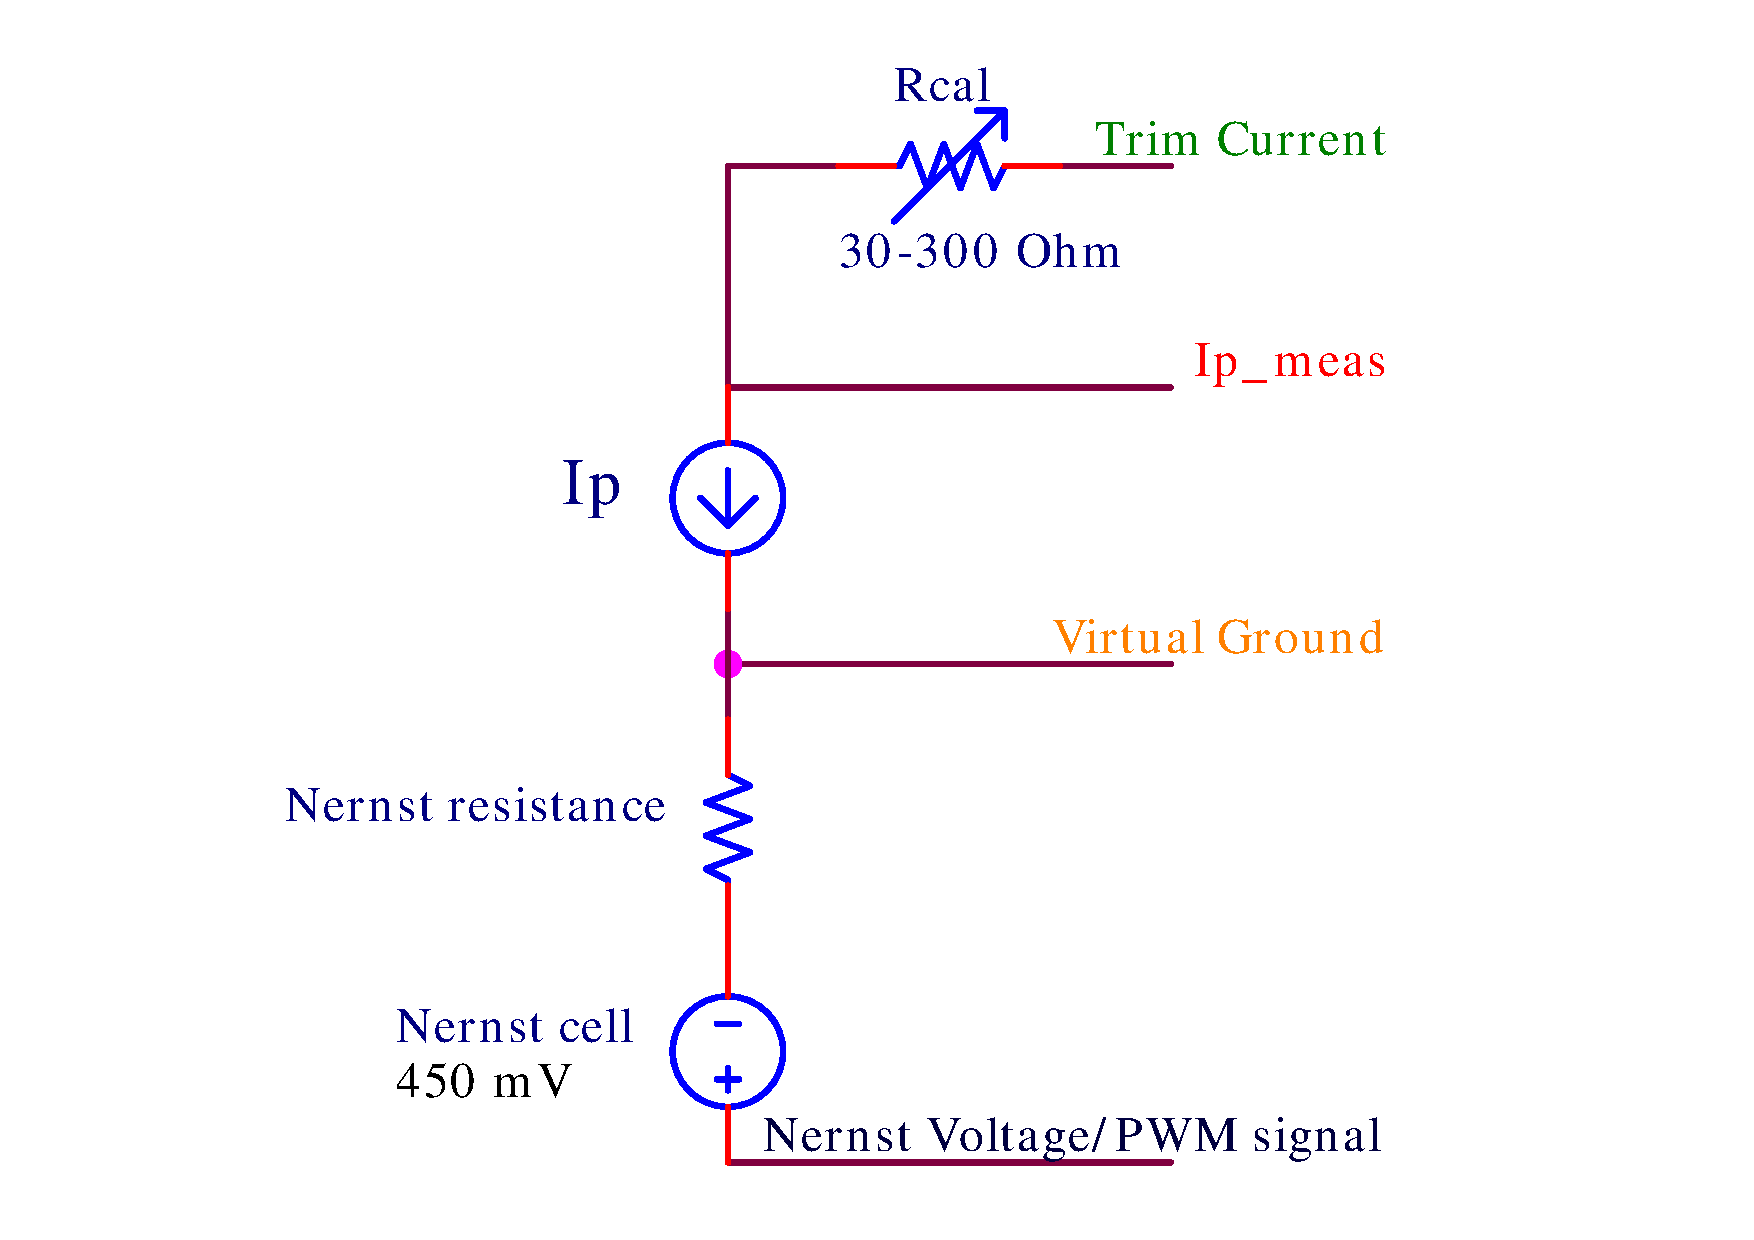
\includegraphics[width = .6\textwidth]{Figures/SCHEMATIC1_lsu49.pdf}
    \caption{BOSCH LSU 4.9 electrical equivalent schematic.}
    \label{fig:schematic_lsu49}
\end{figure}

Figure \ref{fig:schematic_lsu49} shows an equivalent schematic of the oxygen sensor and 4 of its connectors. It does have 6 connectors however, where the 2 connectors which are not shown are for the heating element and is not used in this case. This is because it draws too much current and the sensor is heated up enough by its surroundings in the oven instead.

To control a lambda sensor, its so called nernst voltage has to be held stable at 450 mV relative to its virtual ground, which are both shown in figure \ref{fig:schematic_lsu49}. This voltage is changed depending on the oxygen level and can also be adjusted by the amount of current going through the sensor. Also the amount of current the sensor uses to hold this voltage at 450 mV, tells the lambda value in the air, and from there it is possible to get the oxygen level in the surroundings.


The lambda sensor is a ZrO$_2$ based oxygen sensor, and the nernst voltage builds on the principle discovered by the scientist Walther Nernst~\cite{Exhaust}. The voltage is generated by a partial pressure over a diffusion bar, the voltage occurs from a ionic reaction from the oxygen. This is also why the lambda sensor reacts to other types of substances than oxygen. To assure the sensor only reacts to oxygen, one wants stable substances surrounding the oxygen, like noble gases or nitrogen. When the oxygen is surrounded by more reactable gases like carbon monoxide or hydrogen, it is more likely the lambda sensor gives inaccurate readings~\cite{LSU49}.


But the lambda value varies with the temperature of the sensor and therefore the temperature also has to be calculated. This can be done by sending a \ac{pwm} signal through a known resistance and the nernst cell's resistance to check its impedance by voltage division. Then there is a look up table in the Datasheet \cite{LSU49} to check which resistance corresponds to which temperature. However, when the \ac{pwm} signal is sent through the nernst cell it can't deliver more current than 250 $\mu$A, because of the maximum ratings of the LSU 4.9. Then the voltage drop will most likely be very small within its operating ranges. If this voltage drop would be directly measured by the 10-bit \ac{adc} available on the PIC18F26K22, it would give a bad resolution. To increase this resolution, an instrumental amplifier is used, which amplifies the difference between the \ac{pwm} signal and the signal where the \ac{pwm} signal gets low pass filtered. The gain of the amplifier is then decided to give a good resolution within the operating temperature. Because of this it does not give correct values for lower temperatures, but it should not be a problem because the sensor does not operate correctly in cold temperatures.

The lambda value from the sensor also depends on the pressure from the surroundings. This has to be considered if there is a higher or lower pressure in the oven compared to the atmosphere.

In the datasheet~\cite{LSU49} it is clearly stated that the sensor should be installed within a certain angle to prevent condensation on the sensor, which will prevent accurate readings and also possibilities for damaging the sensor during heat up process. But this sensor is supposed to sit in the exhaust pipe on a car, where it can be a lot of water and high humidity. In this case the sensor will be put in an already preheated oven and therefore it should not be any liquid water that can enter the sensor. Also the most advantageous way to mount the sensor is upwards, because it is mounted in a metal box, with no possibility to mount it on the side or bottom of the box.

%and its position and angle can't be controlled. But because of the very high temperature that occurs in the oven, the possibility for condensation are supposed to be small and therefore the sensors angle hopefully don't have to be considered as much as it would have to be in the exhaust pipe of a car.


\section{Electronic functionality}

In total there will be three differential amplifiers. In this case we use \ac{ic} with pre-built instrumental amplifiers, where you can set the gain with only one resistance. The amplifiers are for the \ac{pwm} signal to measure the temperature, one for measuring the nernst voltage, where it amplifies the 450 mV a few times to reach a higher resolution on our 10-bit \ac{adc} configuration and there is an instrumental amplifier to measure the voltage drop over a 61.9 $\Omega$ resistor to find the $I_p$.


The pump current $I_p$ for the sensor is controlled using a \ac{dac}. The DAC's output is a voltage source, but the resistance after the \ac{dac} is stable and the current is then changed by changing the output voltage from the \ac{dac}. $I_p$ have a low operation swing, and with this follows that the DAC's usable output is about 200 mV. To be able to reach a high-resolution within this output range, one has to select a \ac{dac} with high-resolution itself. The used \ac{dac} is a 12-bit \ac{dac} with \ac{i2c} communication and is an AD5622 \ac{ic} from Analog Devices,~\cite{AD5622}.


By not using the internal heater in the LSU 4.9, there is no need to have access to high voltages and it should make it possible to control the sensor with only 3.3 V. The changes for it to run on 3.3 V, is that the virtual ground has shifted from suggested 2.5 V to about 1.5 V or similar. The important thing is that it is somewhere between 0-3.3 V and that it is possible to reach the wanted voltage ranges from there. In other words high enough to reach the 450 mV over the nernst cell, and low enough so the supply voltage is enough for the pumping current to hold the nernst cell on 450 mV in an oxygen rich environment.




\section{MCU description}

The first choice of \ac{mcu} was the PIC18F26K20 which is the same PIC processor that Electrotech uses for their radio unit, which also is the system we will have to communicate with. However, this PIC processor has only one \ac{i2c} bus and the sensor system requires two \ac{i2c} buses. The sensor system has one \ac{i2c} bus where it is the slave to the radio system implemented by Electrotech and one bus where it is master for the \ac{dac}, used for the pumping current to the sensor. It could maybe be possible to switch one bus between master and slave, but it is easier to change to a PIC processor which has two \ac{i2c} buses instead. A good candidate for this PIC change is the PIC18F26K22, which has similar functionality to the PIC18F26K20, with the difference that it has two \ac{i2c} buses and it has a wider input voltage range of 1.8-5.5 V. The wider voltage range makes it possible to run the sensor on 5 V, is so desired. 

When building the systems to one unit, the complete setup most likely runs on 3.3 V. So when building them together it would simplify the process if the sensor system could run on 3.3 V. This also makes the \ac{i2c} communication between the two systems easier to design, because there is no need for a level conversion.


\section{Meetings}


%There were many meetings early in this project. Those meetings were useful to gather information and discuss what should be done and how things are going to be integrated with each other to achieve a good result.



In the beginning of this thesis, there were many meetings to gather information about how things should work and cooperate. Many technical decisions were made from discussions during these meetings. For example, things like operation voltage, sensor functionality and mechanical design were discussed. Below follows some discussions from the most productive meetings.

\subsection{Meeting in Kalix}% with Electrotech}

Electrotech located in Kalix, is the designer of the radio circuit used to send all measurement data out from the oven during these experiments. Because their radio circuit has to cooperate with the sensor circuit it was crucial to have a meeting to discuss some solutions for the functionality and communication.

The main topics at this meeting were mostly about how the electronics should be integrated with each other and which voltage levels that is most logical to use for especially the electronics controlling the oxygen sensor. The communication between the sensor system and the radio transmitter made by Electrotech will go through \ac{i2c}. As the radio system runs on 3.3V the communication between the two systems will have to be at 3.3 V. Then one has to choose if the electronics for the sensor should operate on 3.3 V or 5 V. 

It is most common to run the sensor with 5 V, but it is possible to run it on 3.3 V. If 5 V is used, a level conversion has to be implemented on the \ac{i2c} lines for the communication between the two systems. If not the \ac{i2c} lines can be connected directly and there would be one less cable between the systems. 

On the other hand in the future if both systems are integrated, the \ac{mcu} that most likely will be used runs on 3.3 V. Then it might be worth to operate the sensor on 3.3 V already now to make the design easier in the future.

%to run the sensor system on 3.3V or 5V. The sensor itself runs mostly on 5V, therefore it would simplify to run the system on 5V as there would not need any level conversion. On the other hand in the future if both systems are put together, their processor will run on 3.3V. Then there will need some level conversion anyhow and it might be good to do them already in this system to simplify the process when putting the systems together.

Regarding batteries, the system will be supplied by Lithium Thionyl Chloride batteries~\cite{TLH-2450}. In earlier test, silver oxide batteries have been used. They tend to fail after about 20 minutes and our measurement are supposed to handle at least 20 minutes, later on it turned out it should sustain 4 hours in the oven. The Lithium thionyl chloride batteries are 3.6 V per cell which means that two batteries have to be put in series together with a voltage regulator to be able to run the system on 5 V.

There were also some discussion on the use of an external crystal should be used for the PIC. But the system has to be power efficient and one way to keep the power consumption low is to operate on a low frequency on the PIC. An external crystal would however also give a higher accuracy on the frequency, but none of the measurement or algorithms need any more time accuracy than the PIC's internal crystal can deliver.


\subsection{Meeting with Fredrik H\"{a}ggstr\"{o}m}

Fredrik has some good knowledge overall about electronics and cars in general. He has also done some previous work with lambda sensors on his spare time and therefore had some valuable knowledge for this project. When sitting down with him and Jonny to discuss how the circuit and measurement should be done, a sketch was done on paper on how I wanted the schematic to look like. Fredrik and Jonny did agreed on most parts, with some inputs on minor changes that they would like to see be changed. For example they would like to see some test points and positions on the board for low pass filters. Fredrik also came up with an idea that we may cut away the heating shield of the lambda sensor completely. This would have to be further investigated if this will be the best approach or not.


\subsection{Phone meeting with Johan Borg}

Me and Jonny talked to Johan Borg over phone to get some inputs on how the system should be implemented in the oven. The sensor can be torn down a bit and it can be possible to tear it down so you add own connectors and in that case the sensor wouldn't be able to reach the water inside the isolation material. The reason to not have the sensor the whole way into the water, is that the sensor have some metallic which is able to transfer the heat quickly and in that case cause the water to boil away faster than expected and the system will not last the entire time in the oven. However the whole sensor can not attain oven temperature because only the outer part are specified to manage high temperatures. By letting the inner end of the sensor be inside the water one would prevent the whole sensor to reach the oven temperature. The inner end and the connectors of the sensor are covered with some thin stainless steel, which according to Johan does not carry heat as well as steel that rust. His thoughts were that it would be good to use the water to cool down the inner parts of the sensor, and that this would not impair the usable time of the system too much. He also suggested that it could be an idea to add an aluminum pipe inside the sensor as the water maybe won't be able to cool it down well enough.

\subsection{Disire meeting}% 27/2}

%The Desire project is split in one hot measurement part and one cold measurement part. So the meeting started with some update within both the hot and cold part, where there were some clarification how the days with the test will go by. After approximately the half meeting, the cold measurement people left and then there were some discussion on mostly how the sensor will be built in mechanical.

The Disire project is split in one hot measurement part and one cold measurement part. For the hot measurement part, which is the only part of the Desire project this thesis belongs to, the main topic at this meeting was how the electronics should be built mechanically, to survive in the oven.

The oven will run for 3 days, giving us the opportunity to run the sensor through the oven 3 times. One time per day. The oven itself shifts boxes forward in several steps, where it is important that the boxes have the right dimensions so each box gets the right step length. At first, this was thought to complicate our mechanical setup, but told from the meeting, Mefos already have a box that would fit our need. This box is then re-used for each test run. There are restrictions in the datasheet on how to place the Lambda sensor, it states that is should be pointing downwards. But the box at Mefos removes that opportunity and it has to be placed upward. The reason it should be placed downward is because of condensation water, but it is highly unlikely that there is any condensation water in the oven.

%The plan was also to fill the inner part of the box with water absorbing flower foam, but because the box that is now used is waterproof and will always stand upright, there might be possible to fill the box we only fluid water. However it is not sure it will be the best method to fill it with water. After the meeting people from Mefos and Electrotec joined me and Jonny to my office and took a look at the prototype that was built so far.

The plan was also to fill the inner part of the box with water absorbing flower foam, but because the box that is now used is waterproof and stands upright all time, it might be possible to fill the box with only fluid water. This might not be the best solution though, as water inside might be very unstable during movements.



\makechapter{Method}{Method\label{ch3}}
\section{Development setup}

\subsection{Sensor setup}

Heating up the sensor is crucial for it to work and this is done by the oven during the real test. But when developing the electronics and software there is no access to any oven suitable for this. Then it is heated up with its internal heating element instead. This is done with a power supply, which is manually adjusted for the sensor to achieve the correct temperature. The sensor works on 7.5 W nominal \cite{LSU49}.

The operating temperature of the sensor is 780 $^\circ$C. Thus, the mounting and the metal surrounding the sensor are also warm when the sensor is heated up. To avoid any burn damage and keep the hot sensor away from sensible equipment, a vise holds the sensor in place, mounted as shown in figure \ref{fig:lambda_bench}.


\begin{figure}
    \centering
    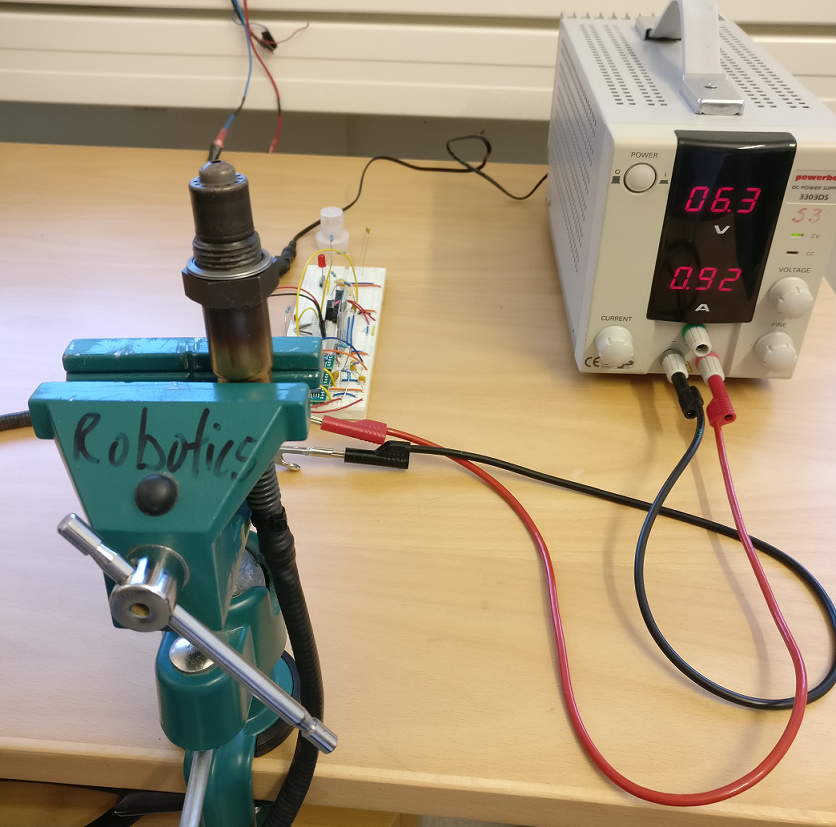
\includegraphics[width=.8\textwidth]{Chapter3/Figures/lambda_bench.png}
    \caption{Lambda sensor mounted to a vise.}
    \label{fig:lambda_bench}
\end{figure}


\subsection{Setup for programming}

Initially a PIC18F26K20 was intended to be used as \ac{mcu}. This is the same \ac{mcu} used in the radio system developed by Electrotech. However, with the need of two different I2C connections and to avoid bit banging it was later changed to a PIC18F26K22~\cite{PIC18}. Bit banging is a software technique for serial communication, when no dedicated hardware is available. This PIC is similar to the first one, but one difference is that it has two \ac{i2c} protocols. The processor was first ordered with \ac{dil}, this to get more familiar with them and it made it possible to connect them on a breadboard, which worked as a development board in this case. The PIC requires a separate device for programming the device. An ICD 3 (In-Circuit Debugger) is the link between the PIC and a Windows platform, it can be used for both programming and debug most of the PICs and was suitable for this project~\cite{ICD3}.





\section{OrCAD simulations}

\begin{figure}
    \centering
    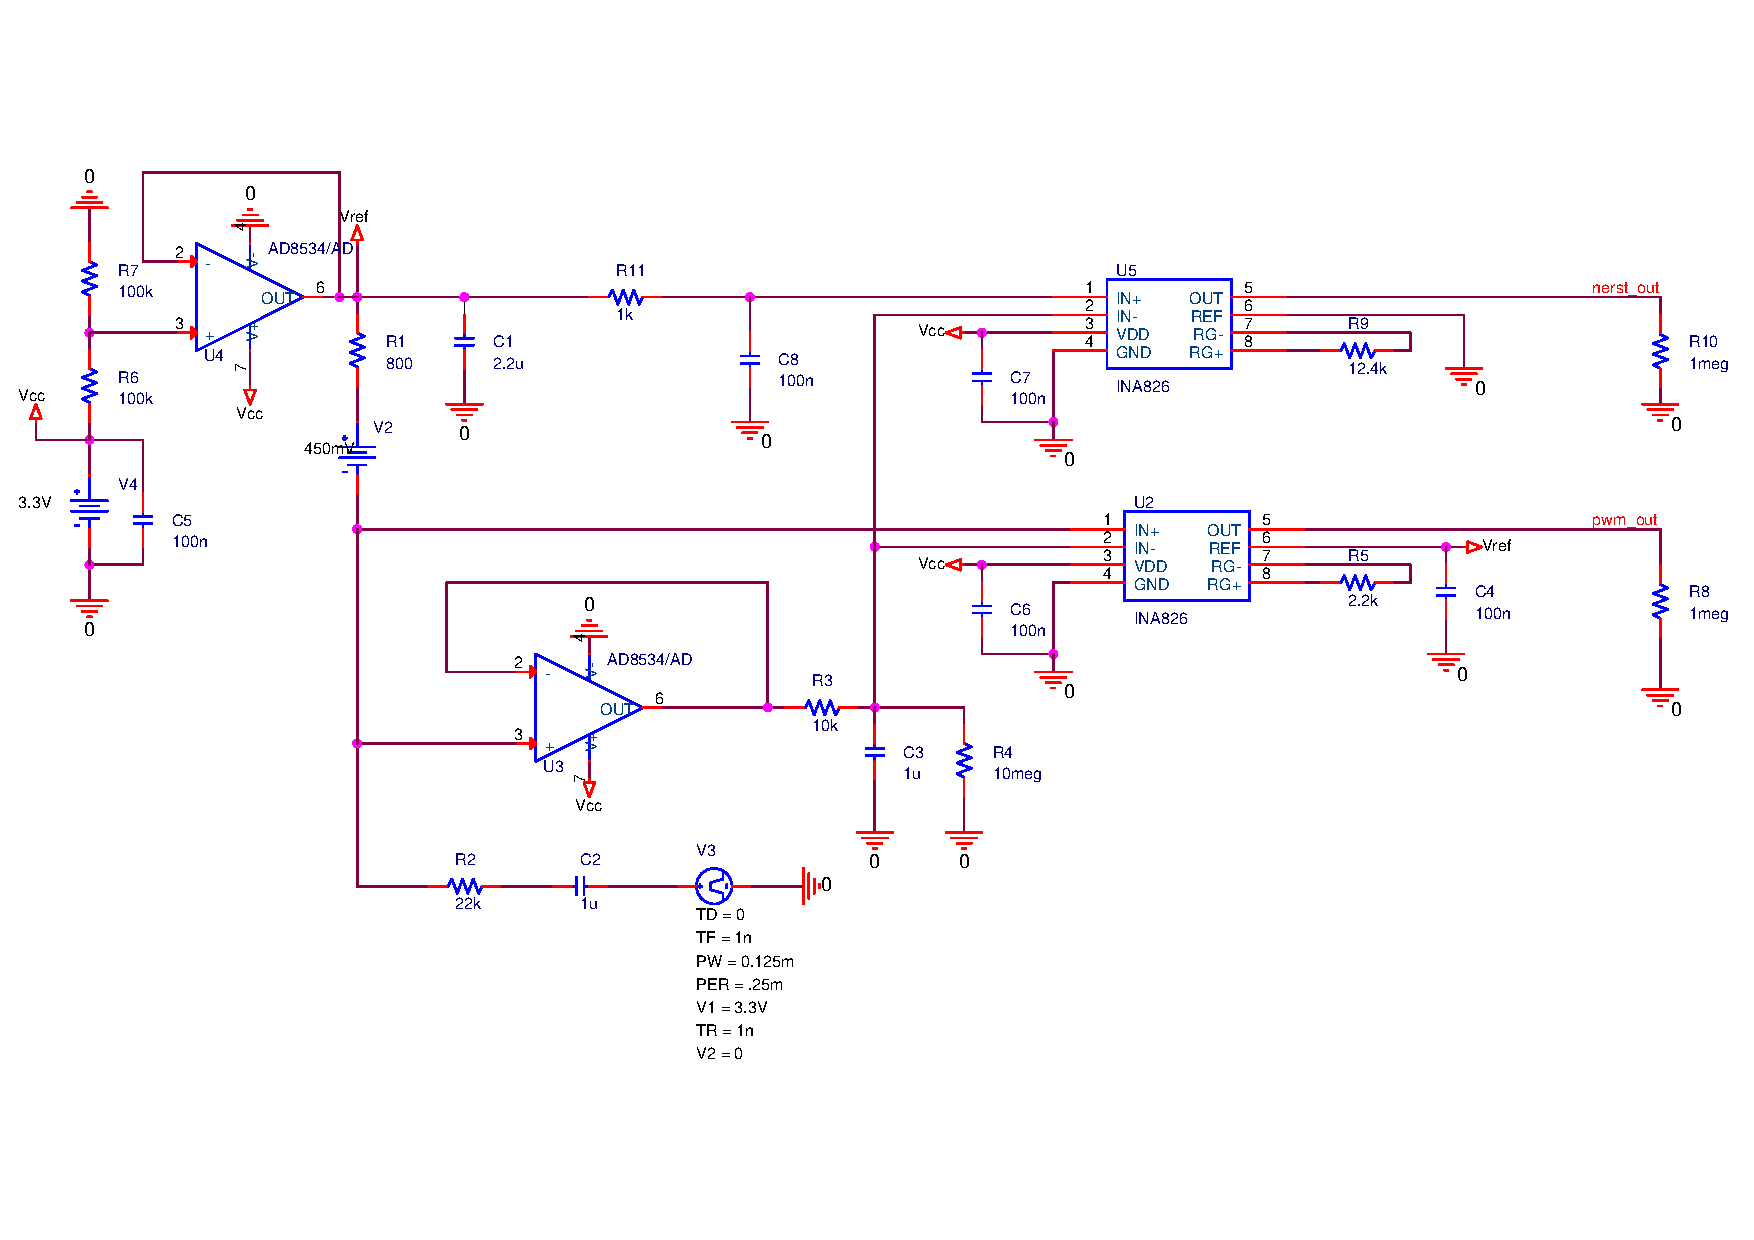
\includegraphics[width = \textwidth]{Figures/SCHEMATIC1_orcad.pdf}
    \caption{OrCAD schematic for nernst cell and instrumentation amplifiers used for measurement.}
    \label{fig:schematic1_orcad}
\end{figure}


By assuming that the sensor was in its operation point during the simulations in OrCAD, the pump-current could be neglected. This simplifies the simulation model and the nernst cell then acted like a voltage source stable at 450 mV. After these simplifications, the schematic looked like figure \ref{fig:schematic1_orcad}.


Over the nernst cell there are two measurements which are of interest. Firstly, one wants to measure the voltage drop over the cell, which is stable at 450 mV if the current regulator behaves as expected. An instrumentation amplifier takes the voltage difference over the nernst cell and amplifies it about 5 times to get a higher resolution on the 10 bit \ac{adc} pins available on the PIC.

The second measurement of interest is the resistance over the nernst cell. Because the cell is held at a constant \ac{dc} level of 450 mV, this measurement is instead done by doing a voltage division of an \ac{ac} signal. This \ac{ac} signal is generated by a \ac{pwm} signal from the PIC, and by supply it to a known resistance and the nernst cell in series, the resistance is calculated by measuring the voltage level between the known resistance and the nernst cell.

The first plan was to run the sensor on 3.3 V because of simplifications in the future if the sensor electronics are integrated in same electronics as Electrotech's radio transceiver. However, because of some battery limitations it was later changed to run on 5 V although all simulations are for 3.3 V.

%Because the temperature is measured with a PWM signal and the temperature in the oven will be kind of stable for long intervals, the temperature will only have to be measured now and then with a high sampling period. With this thought it was first supposed to only send a PWM signal in bursts when the temperature were going to be measured. However this may cause some problem and inaccurate readings, because the PWM signal goes from 0-3.3V it will generate a DC level on about 1.65V and when the DC level are implemented in the circuit it will take some time for the circuit to become stable and no readings should be made during this stabilising process and this may cause problem because the nernst cell will have to be continuously read to be able to control the current so the nernst cell will have a stable voltage.

\subsection{PWM signal}

It is expected to have a stable temperature of the sensor in the oven. Only the oven is heating up the sensor, so the temperature changes are most likely small over time, compared to if the heating element heats the sensor. Thus the first thought was to only measure the temperature in long intervals, by sending a \ac{pwm} signal in burst while measuring the temperature. Then, the amplitude of the \ac{pwm} signal represents the nernst cell resistance, which represents the temperature of the nernst cell.

However this may cause some problems and inaccurate readings, because the PWM signal goes from 0-5 V. It generate a DC level of about 2.5 V and when the DC level is supplied to the circuit, it takes some time for the circuit to become stable and  no readings during this stabilising process are preferable. This may cause problems because the nernst cell is continuously read, so for the current regulator for the pump current which holds the nernst cell voltage stable, there is a time frame with unexpected behavior.


One alternative is to send the \ac{pwm} signal during all time the system is active and taking measurements. But the \ac{pwm} signal is causing a noisier signal over the nernst cell and that can disturb the nernst voltage measurements.


Because of this issues both methods were tested to be sure which would give the best accuracy of the sensor readings.


\section{Temperature measurement on prototype board}

After the OrCAD simulations \ac{ic} adapters to build the circuit used for the temperature measurement over the nernst cell on a breadboard became useful. Before connecting the real lambda sensor to the breadboard a resistor of 220 $\Omega$ simulated the nernst cell resistance to see if the \ac{pwm} signal was correctly divided and amplified in the circuit. At first, the output signal which was connected to an \ac{adc} pin was just noisy and there was no characteristic of a \ac{pwm} signal. The decoupling capacitor on the virtual ground was then replaced by a bigger capacitor because this signal was also a bit noisy. After the change it was easy to see the measured \ac{pwm} signal. However it was still a bit noisy and one has to consider that when building the final board if it should be increased even more or if there is other reasons for the noise, or if it decrease only by building it on a PCB, which makes everything tighter.

The test resistance was then replaced with the lambda sensor and the sensor was heated with a power supply, where the voltage was controlled to not exceed the recommended heat up restrictions stated in the datasheet for the lambda sensor. When the heating element was supplied with 6 V, the measurement still showed the maximum \ac{pwm} output signal, going up to 6.4 V it decreased so the amplitude stated an resistance a bit below 1k$\Omega$, which represents an internal temperature of about 650 $\circ$C. The output signal is still a bit noisy, so to get a more accurate value, some more noise has to disappear.


\section{Breadboard run with major parts of the sensor circuit}

After being able to measure the temperature and communicating with the \ac{dac} through \ac{i2c} some tests were done on the sensor with most of the components mounted on a breadboard. The \ac{dac} could be controlled with the phone through a bluetooth terminal and the HC-06 module to the PIC18's eusart pins. It was controlled by either writing a "+" or "-" were the signs represented small steps up/down for the voltage. After some debugging and errors it turned out that the voltage drop over the nernst cell went the opposite way than expected. This caused the value for the voltage drop over the nernst cell to remain at 0 V when it in fact was increased. The reason was found to be that the differential amplifier stage was implemented with reversed connections on IN+ and IN-, which was later corrected.

\begin{figure}
    \centering
    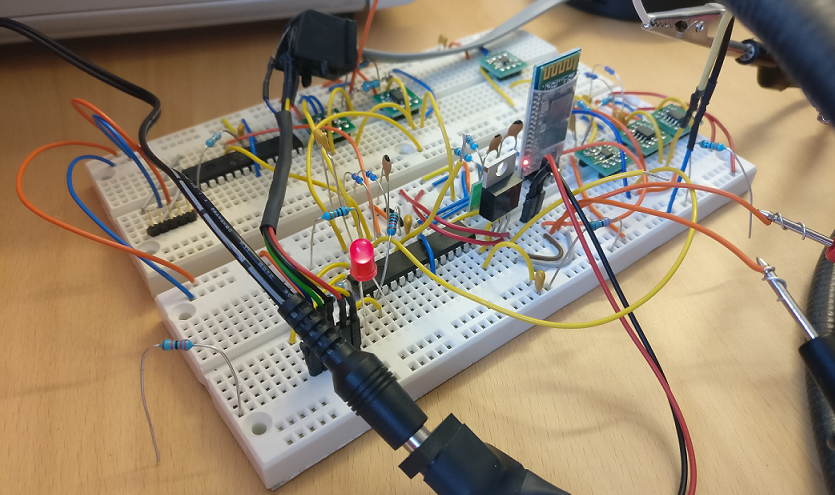
\includegraphics[width=.6\textwidth]{Figures/breadboard.png}
    \caption{Most of the functionality connected and tested on a breadboard.}
    \label{fig:breadboard}
\end{figure}


\section{Schematic description}

\subsection{Power supply}

There are two transistors used for power switching as shown in figure~\ref{fig:supply_schematic}. One switch is controlled by the PIC processor and the other switch can be controlled by an external device.

This second switch was meant to power down all supply and therefore end up with almost no power consumption when the power was cut off. It was meant to be connected to the radio module, which could then decide when to power on or off the sensor system. This second switch was bypassed however, so the PIC always had access to power supply. Sleep mode was instead invoked when no I2C command was received from the radio module.

The PIC then controlled the first switch which it turned off before entering sleep mode and switched on when it wake up and started to take measurements.


\begin{figure}
    \centering
    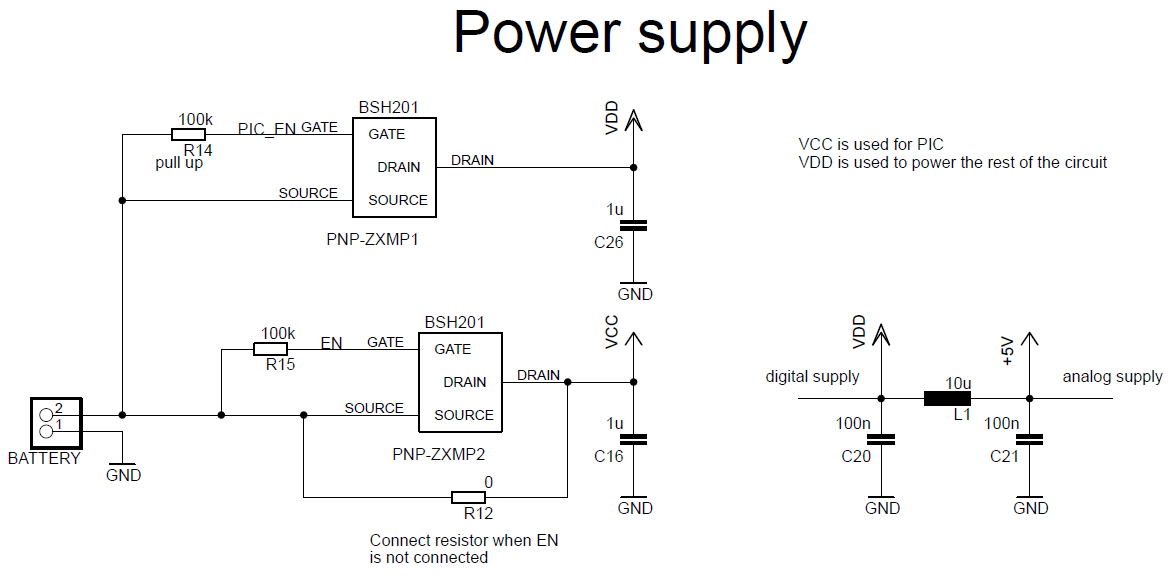
\includegraphics[width = \textwidth]{Chapter3/Figures/supply_schematic.png}
    \caption{Power circuit for PCB.}
    \label{fig:supply_schematic}
\end{figure}


\subsection{DAC for current regulation}

The DAC controls the current supplied to the lambda sensor and its schematic can be seen in figure~\ref{fig:DAC_schematic}. It is provided with a LC-filter on the output, where a ferrite inductance is placed over the gap between the digital and analog ground. The device is a 12-bit AD5622~\cite{AD5622} DAC supporting I2C communication, where the 12-bit value is linearly distributed between ground and supply. The capacitors added to the I2C lines are optional and was added because they stabilised the communication when the system was connected to a breadboard. It was not found necessary to use them on the final \ac{pcb} design.


\begin{figure}
    \centering
    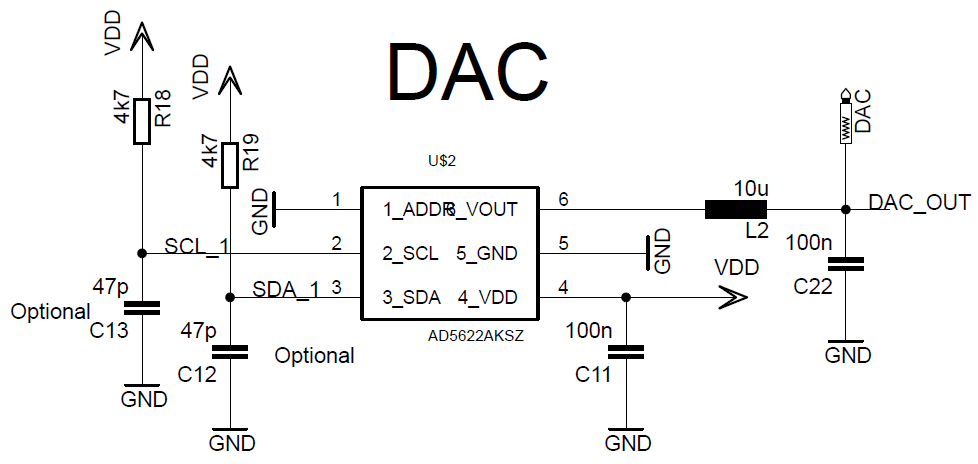
\includegraphics[width=.9\textwidth]{Chapter3/Figures/DAC_schematic.png}
    \caption{Schematic for the DAC controlling the current to the lambda sensor.}
    \label{fig:DAC_schematic}
\end{figure}


\subsection{Operational amplifiers used as impedance buffers}

In total three operational amplifiers were used, and the schematics for them is seen in figure~\ref{fig:OPamp_schematic}. All three were connected to have unity gain and used as an impedance buffer. It is almost the same operational amplifiers, with the difference that AD8539 comes with two op-amps in one package.


When setting the virtual ground, two resistors is used as a voltage divider. Then this node is connected to a high impedance input pin on an op-amp which acts as an impedance buffer.


The pin named nernst cell (RE+)~\cite{LSU49} will hold both a \ac{dc} and \ac{ac} signal. To get a clean \ac{dc} signal, the \ac{ac} signal is low-pass filtered by an RC-filter. Before the signal enters the RC-filter, it goes through an op amp used as an impedance buffer. So the RC-filter does not have any influence on the original signal.


\begin{figure}
    \centering
    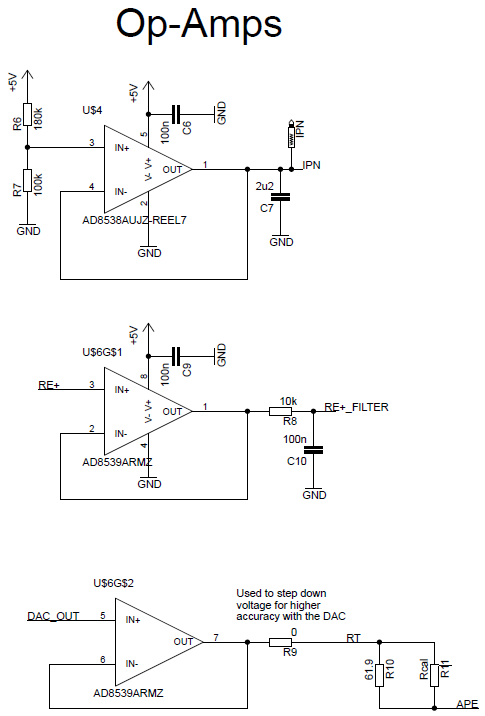
\includegraphics[width=.7\textwidth]{Chapter3/Figures/OPamp_schematic.png}
    \caption{Schematic for the three OP-amps used as buffers.}
    \label{fig:OPamp_schematic}
\end{figure}


\subsection{Instrumentation amplifiers}

The instrumentation amplifiers hold a circuit of three operational amplifiers within the \ac{ic}, where they connect in such a way that it takes the difference between two input signals and amplify it with a gain depending on one resistance. The output signal will then be the amplified difference between the input signals added to the reference point which the user set to a level between ground and supply on the reference pin.

The differential signals compared with an instrumentation amplifier, in this case, are the nernst voltage compared to virtual ground and the pump current, which is done by measuring the voltage drop over a 61.9 $\Omega$ resistance. The third amplifier compares the PWM signal entering the nernst cell with a low-pass filtered signal of the PWM signal. This to be able only to amplify the amplitude of the PWM signal before measuring it using an ADC pin.

In figure \ref{fig:INA_schematic}, the resistance connected between RG1 and RG2 on each amplifier sets the gain~\cite{INA826}, where the gain can be calculated by,

\begin{equation}
    G = 1 + \bigg(\frac{49.4~k\Omega}{R_G}\bigg).
\end{equation}

The reference pins on the amplifiers are connected to different points, depending on which signals that are compared. The nernst voltage is always supposed to be positive, and if so then the reference pin is connected to ground because then the output signal is always above the reference point.

The pump current can be negative, and therefore the reference pin is connected to virtual ground, which allows the instrumentation amplifier to amplify both a negative and positive difference on the input signals. The reference pin for the PWM amplitude amplifier also connects to virtual ground.


\begin{figure}
    \centering
    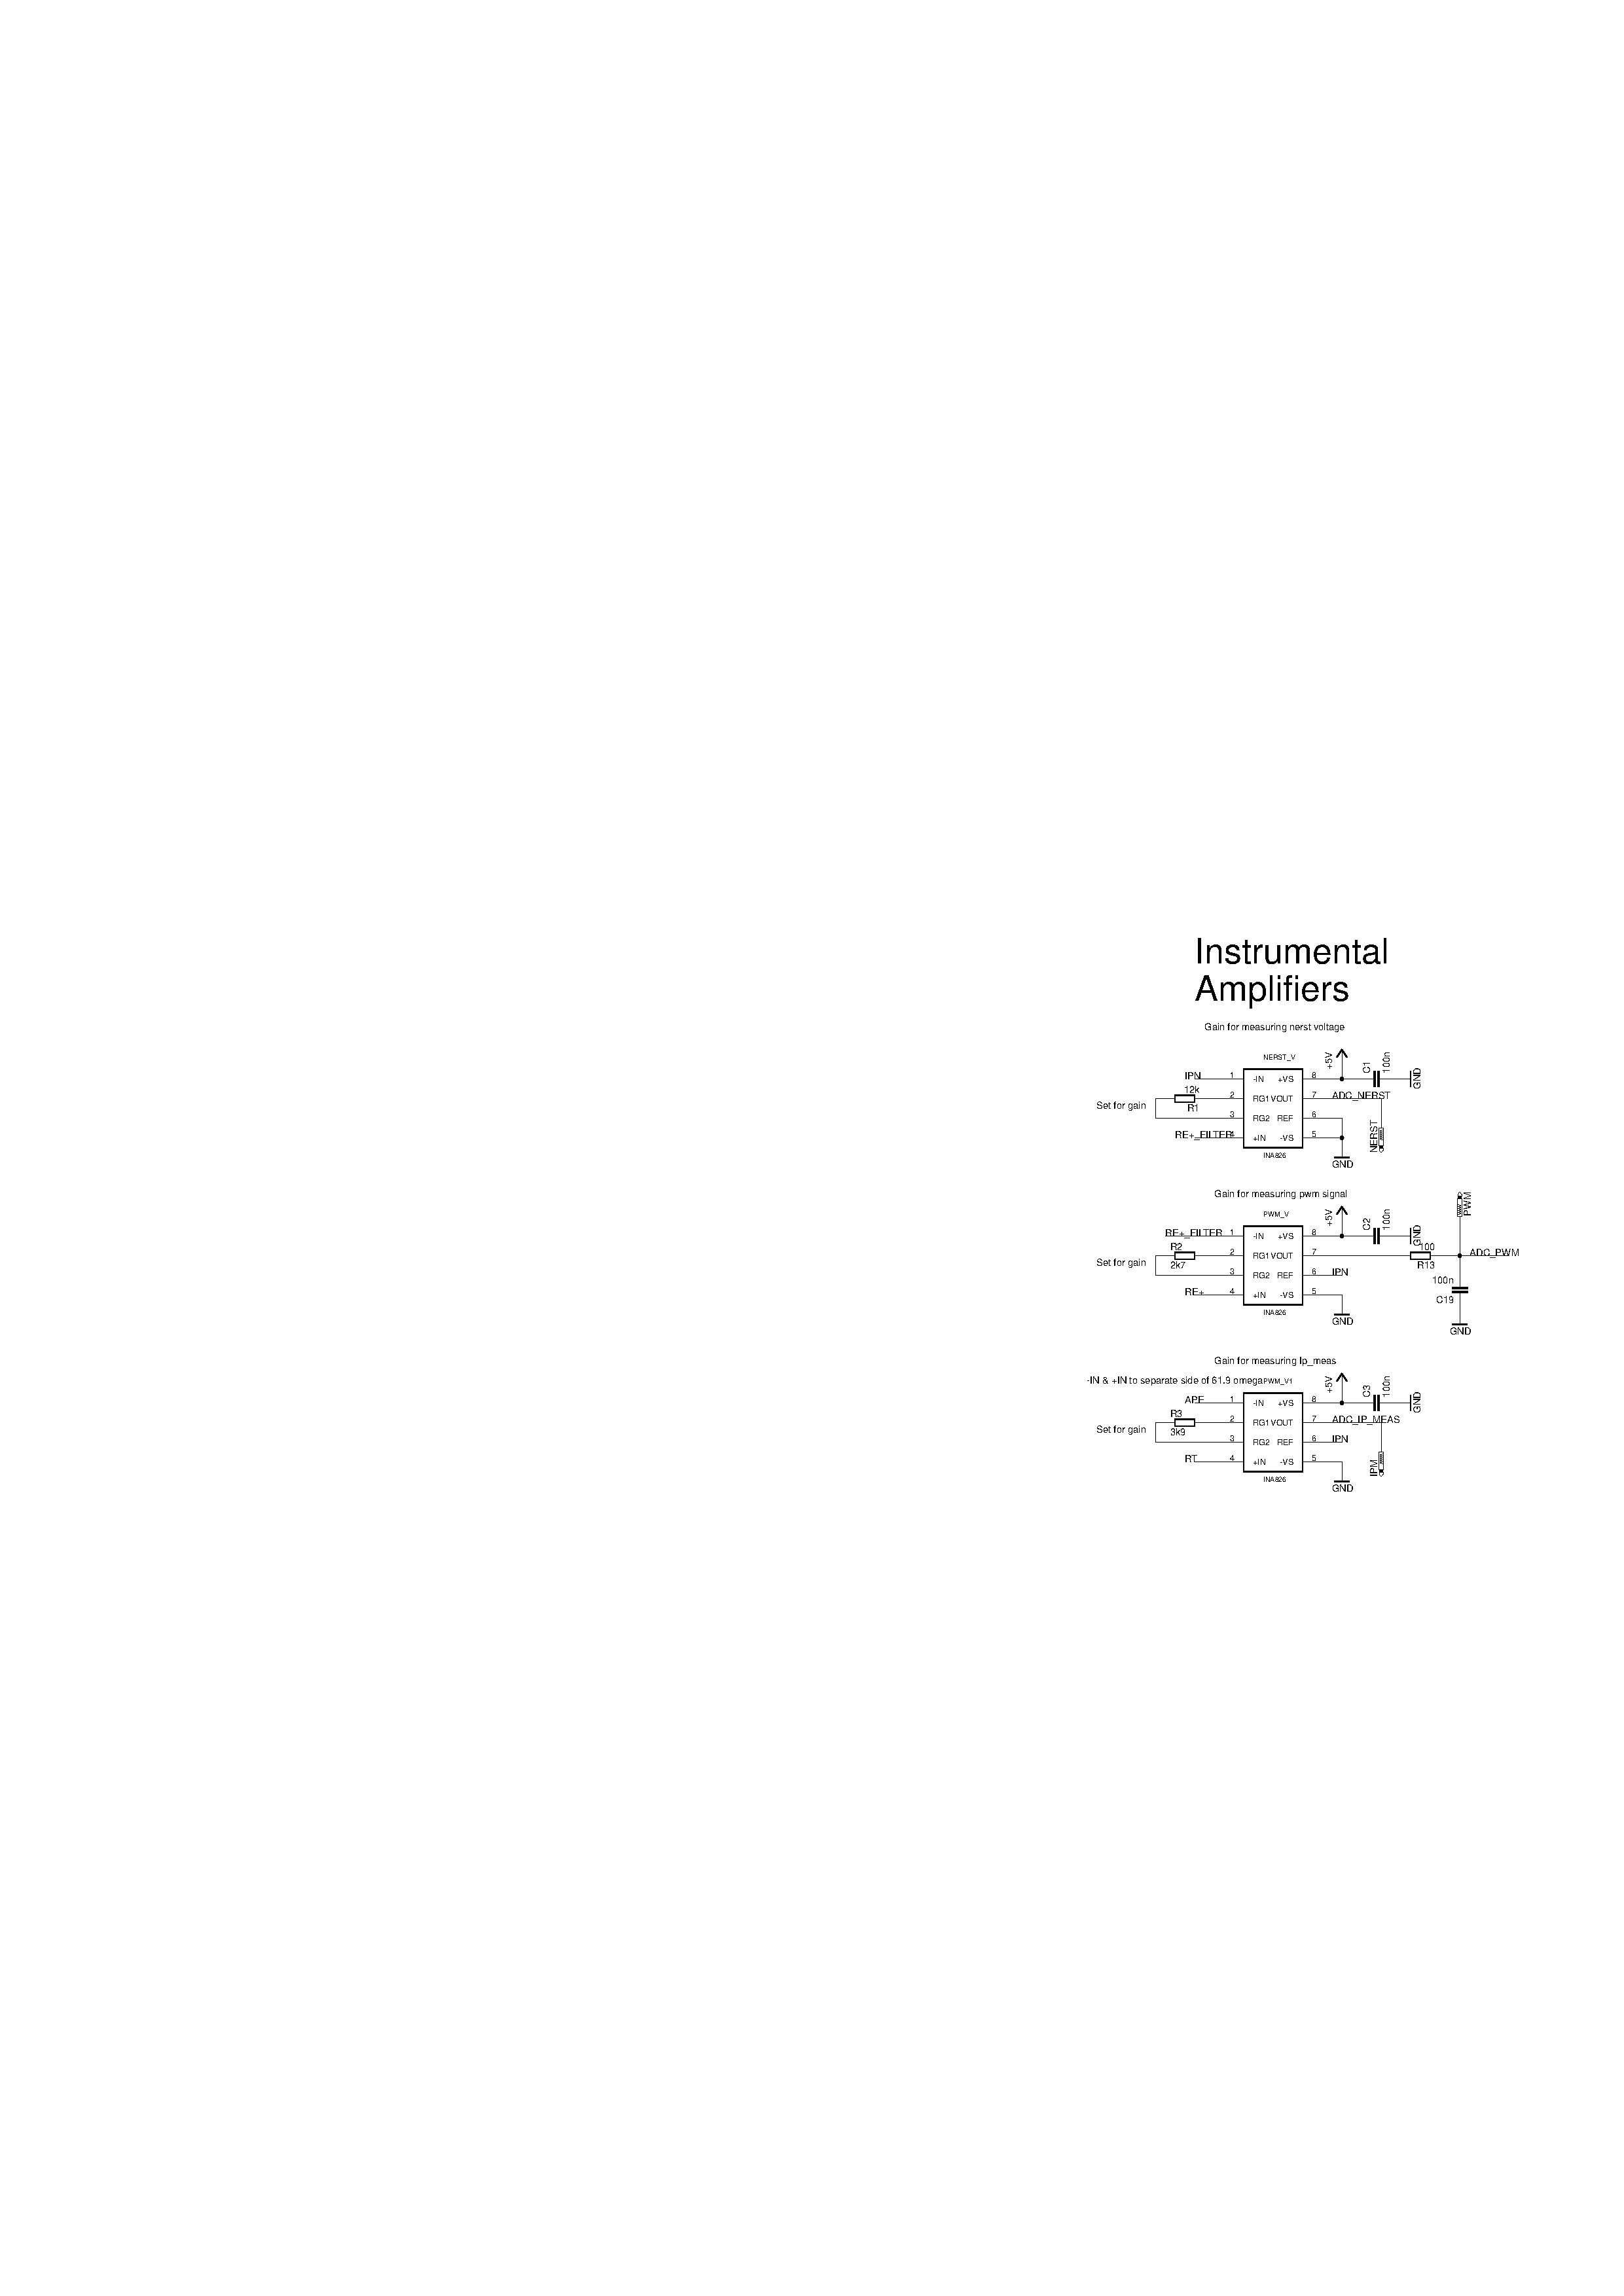
\includegraphics[width=.7\textwidth]{Chapter3/Figures/instrumental_schematic.pdf}
    \caption{Instrumentation amplifiers used for nernst voltage, pump current and temperature measurements.}
    \label{fig:INA_schematic}
\end{figure}


\begin{figure}
    \centering
    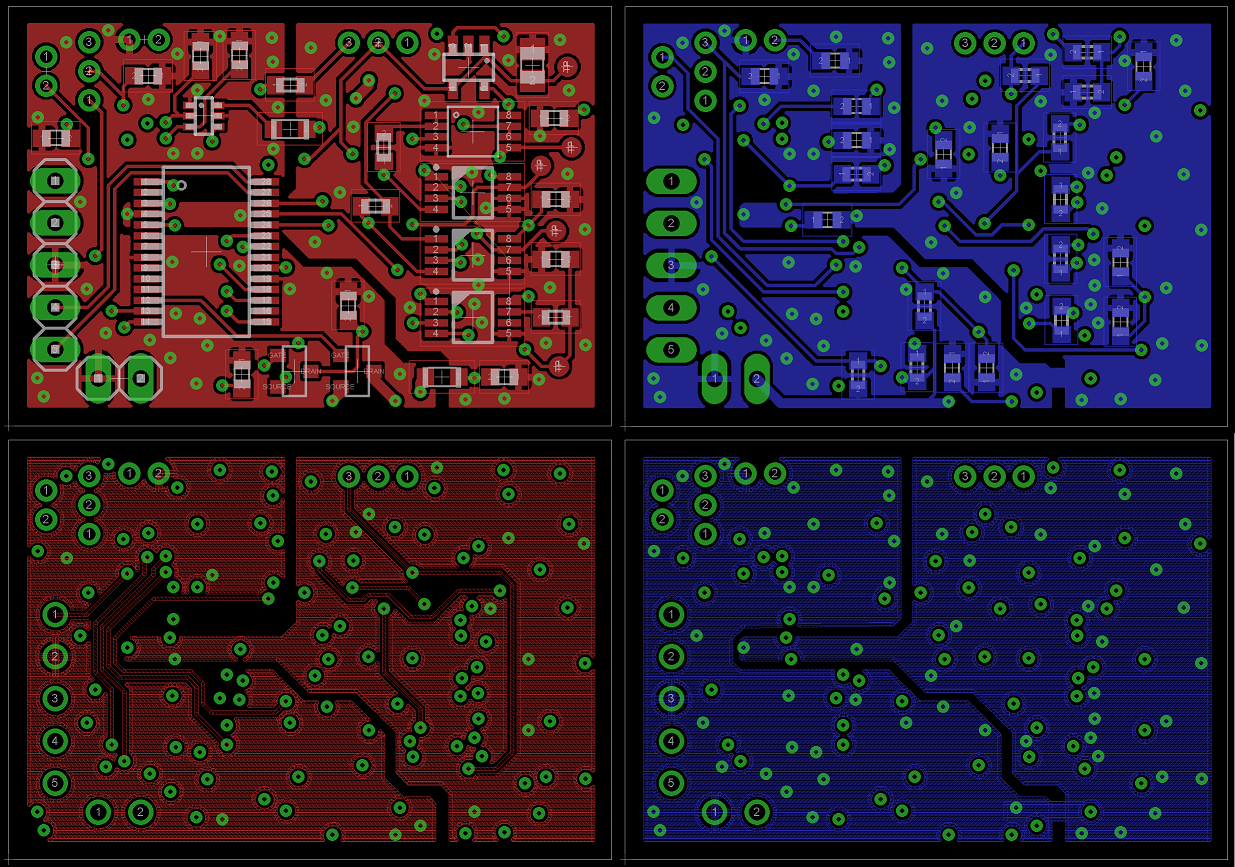
\includegraphics[width = \textwidth]{Figures/PCB4layer.png}
    \caption{All four layers of the PCB in Eagle. Red represents the two top layers and blue is the two bottom layers.}
    \label{fig:PCB4layer}
\end{figure}


\section{PCB design}

After simulating the circuit and running it on a breadboard, it was implemented as a schematic in Eagle~\cite{EAGLE}. The circuit already had some minor patches on the breadboard, which was taken care of on the schematic design in Eagle. The analog part of this circuit is the major part and also the most critical part to be able to get high accuracy on the measurement. A full schematic for the final \ac{pcb} design is found in appendix~\ref{appB}.

\subsection{Separating analog and digital signals}

The sensor system consists of mostly analog circuits. Here it is important that the analog signals don't get disturbed by the digital signals, to be able to have smooth and clean analog signals sent to the PIC. By splitting the ground plane into two parts and connect them at one node isolate the analog part. This method is called star-ground where several ground planes are connected just in one node. The analog part of the ground plane covers all analog circuits and the pins on the PIC where the analog signals are being handled.

This separation is done by doing a cut in the copper plane where all digital signals placed on one side of the cut and the analog signals placed on the analog part of the ground. However, one small path between the ground planes allows the analog and digital ground to be still connected to each other, see the dark blue picture in figure~\ref{fig:PCB4layer}. All pins used as analog pins on the PIC are selected, so they are close to each other, this because the PIC covers both the analog and the digital ground. So by having the analog pins close to each other, it simplifies the splitting of the ground plane.


There is also important to have a clean supply voltage, in particular for the analog circuit. To achieve clean and accurate analog signals is as little noise as possible on the analog supply wanted. The voltage from the battery is split in two. One supply goes directly to the digital voltage supply, and the other supply is connected through an LC-filter to prevent noise raised in the digital part to reach the analog part.

Also, all signals going from analog to digital part have a series resistance to prevent noise, this resistor is placed over the gap between the analog and digital ground.

\subsection{Dimensions}

Because there are some space limitations in the oven, it is beneficial to have a small \ac{pcb}. Therefore a \ac{pcb} with four layers is designed, because it makes it easier to place components on both sides and still have a good ground plane. On the two layers in the middle, there is one ground layer and one supply layer. In figure~\ref{fig:PCB4layer} the dark blue layer is the ground layer, and the dark red layer is the supply layer. The ground layer is free from traces. Keeping the ground layer free from traces allow the signals have the shortest possible circuit. The signals are then less likely to pick up noise. The outer dimension of the \ac{pcb} is 26x37 mm.

\subsection{Connector}

The following connections are available on the PCB,

\begin{itemize}
    \item Power
    \item Programming
    \item Lambda sensor (LSU 4.9)
    \item \ac{i2c} communication
    \item \ac{usart} communication
\end{itemize}

For the power and programming connectors, which is visible in the top corner in figure \ref{fig:monterad_PCB}, it use standard pin-header connectors with 2.54 mm pitch. This type of connection makes it easier to connect, disconnect and program the device. The device is under a development process, and that's why this simplicity is especially wanted. So if another \ac{pcb} would be designed as a finished product, these connectors would most likely be smaller.


The connectors for the lambda sensor, \ac{i2c} communication and \ac{usart} communication have all the same size on the connectors. This connection was not a good idea for the lambda sensor, since its wires are thicker than the connector holes and thus makes it a bad design. For the \ac{i2c} communication and \ac{usart} communications it was suitable. It could however be designed with a bit wider solder pad to simplify the soldering process.


\subsection{Component size}

Most of the passive components are 0603 components. 0603 tells the components dimensions in mills. 0603 components are small enough not to take too much space on the \ac{pcb}, but big enough to be soldered by hand with not too much of a hazard.

Most of the ICs used were available in both \ac{soic} and \ac{sop}, the \ac{sop} was selected to keep the size down. It should be possible to find a suitable transistor with a smaller package however.


\begin{figure}
    \centering
    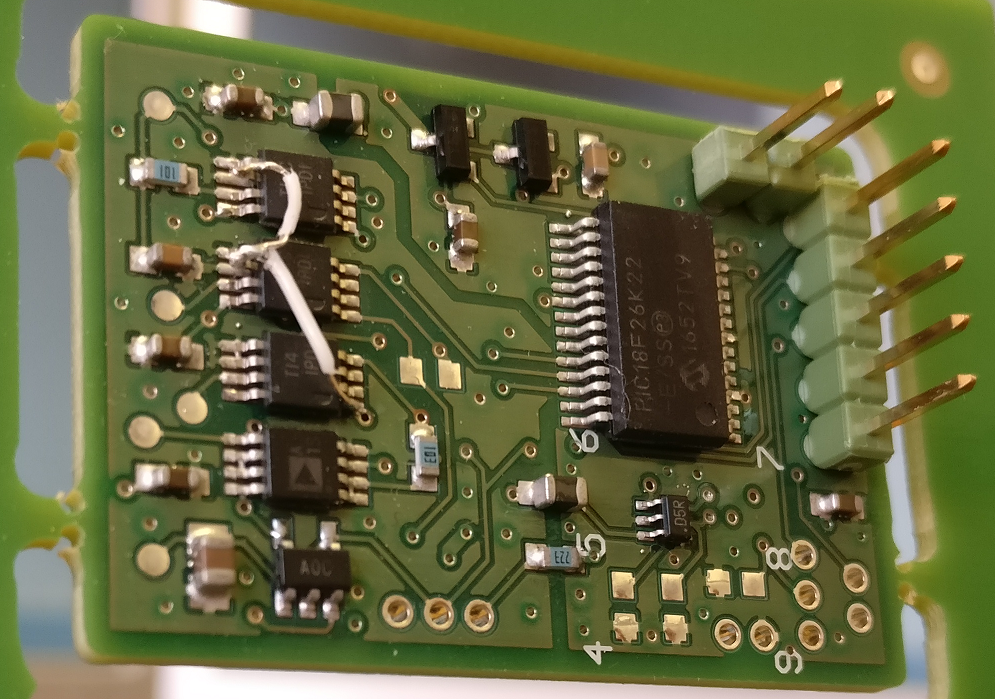
\includegraphics[width=.6\textwidth]{Figures/PCB_monterad.png}
    \caption{Mounted PCB.}
    \label{fig:monterad_PCB}
\end{figure}


\section{Operating voltage}

The operating voltage for the sensor was first decided to be 3.3 V. The system was then also designed for this voltage, but it didn't manage to run on a lower volt than 3.3 V in an oxygen rich environment. But Electrotech had some concerns that the used batteries which, could drop down below this limit. Because of this reason, two batteries were put in series and connected to a 5 V voltage regulator.

This change seemed not to be any problem because all electronics used for the sensor system were designed to handle up to 5 V. The system also uses the \ac{fvr} built into the PIC, to compensate for an eventual difference in supply voltage. However, the gain from the pumping current measurement and nernst voltage measurement was constant. With this follows that the voltages which are to be measured, don't follow the increment of the supply voltage from 3.3 V to 5 V. This gives a lower accuracy on these measurements if the gain is untouched and they are limited by the 10-bit \ac{adc}, which follows the supply voltage. 


\section{Communication between Radio system and Sensor system}

Electrotech has been adding space for four wires to connect to their system for the \ac{i2c} communication. Two wires used for the actual communication, one wire to have a common ground and the last wire for level conversion on the data and clock lines. However, since the system seemed to most likely run on 3.6 V unregulated, there would not be any need for a level conversion, because both systems would run on same supply level in this case and it would give us the opportunity to run on the same battery. But the supply was later changed to 5 V, and the level conversion was then needed.

\subsection{Communication protocol}

Electrotech gave us some opportunity to decide how we want the communication to be in some sense. The sensor system has to wake up from sleep or idle mode through an \ac{i2c} command. Then the radio system is pulling for data where we set up how the pulling should be implemented and then set up how we want to send the data. Then the data is then sent to their radio antenna.

The communication starts when Electrotech sends a start command (0x01). This command wakes up the sensor system which then responds with (0xff), which represent that no data are available yet. The sensor system stays awake and measures as long as Electrotech repeatedly sends request one time per second. When the sensor system has stabilized, it responds with 48 bits of data. 16-bits each for the oxygen concentration, sensor temperature and the nernst voltage.



%\section{Trip to Kalix 20170315}
\subsection{Test run in Kalix}

When both parts have been working on the communication on their own, it was time to verify that it worked as expected. It was tested in Kalix, and it didn't work from the start. By using an oscilloscope with built in \ac{i2c} decoder, able to display what the communication looked like on the oscilloscope was a useful debugging tool.

At the end of the day, the I2C communication worked in some sense. It looked correct on the oscilloscope, but some error in the software which not acted as expected. By doing an exchange of electronics, so both parts had access to all electronics used in the experiments, made it possible to work further from a distance. Hex-files of software could then be sent from one part to the other, who then reprogrammed their device.



%The main goal with this trip was to check if the communication between the sensor system and Electrotech's radio unit worked as expected. As mentioned before the communication protocol used was I2C. There were some struggle before it worked as expected with some minor bugs from both part. However, the one who was responsible for the communication from their part, had an oscilloscope on his office, which were able to read I2C protocol and it was a great source for the debugging process. At the end of the day we manage to setup the communication so it looked good on the oscilloscope, but Electrotech didn't manage to read the data and send it further by radio. This was most likely some bug from their part and they are going to send a software update when it is fixed. Because we did some exchange of hardware there will be easy to just send some software update to test when it is fixed.

\section{Tests performed in oven}

There have been three tests in an oven in total. The first test, which is also the biggest test, was in an oven where all the electronics were inside the oven during the test. This test lasted for about 2 hours, and all the electronics were surrounded by water for cooling properties, while the sensor was pointing out to the oven. 

The other two tests have been in a small oven. Here, only the sensor functionality was tested. In other words, the electronics were outside the oven and only the sensor was exposed to the oven. These tests were done to see how the sensor behaved in this kind of environment and to verify that the electronics were functioning.




\section{Building process in Kalix}

\subsection{Waterproofing of electroncis}

%After some concern however the sensor oxygen electronics will be able to run on 3.6V, the voltage level was increased to 5V. Because all electronics were design to handle some level shift without giving wrong measurement data, this wasn't a problem and all components were rated for 5.5V or more. The critical part by doing this was the level-shift on the I2C communication and this was implemented by Electrotech.

Water surrounded the electronics during the tests, which was used for cooling. Then the electronics were covered with some waterproof epoxy to keep all water away from the electronics, so the water only fulfills its cooling effects.

After testing all functionality and power consumption, the electronics were soldered together and tested before placing it in plastic boxes. The communication didn't work at first, but it turned out that data and clock lines were switched on the I2C communication. Figure \ref{fig:electronics_box} shows how all electronics placed in a plastic box, which later on was filled with some waterproof epoxy. The box was used to keep the epoxy in place before it hardened.



\begin{figure}
    \centering
    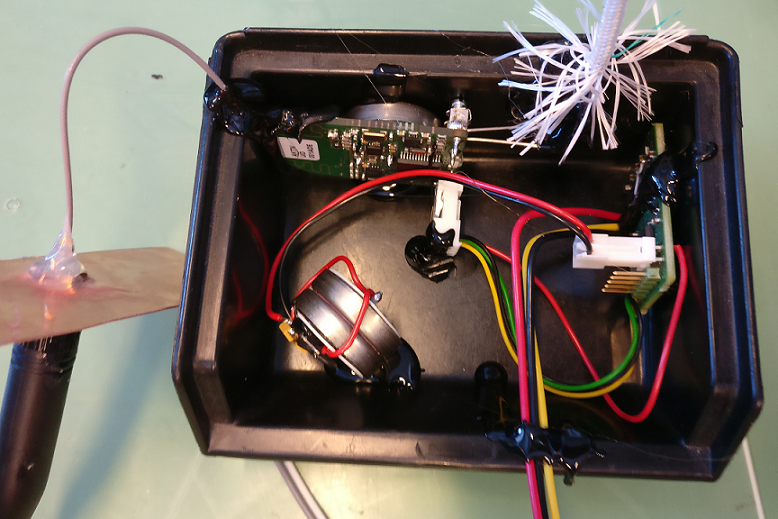
\includegraphics[width=.8\textwidth]{Chapter3/Figures/electronics_box.png}
    \caption{Electronics in plastic box before covered by epoxy.}
    \label{fig:electronics_box}
\end{figure}


\subsection{Mechanical design}


In figure \ref{fig:mechanical_construction} one can see how the system look before water surrounded it. In the figure, the system is upside down, where it during the test is flipped and surrounded by water. The white plate is isolation material and is the top of the system. It has one hole for the lambda sensor, one hole for thermocouple and some smaller holes where water vapor can escape.


All electronics and sensors were mounted to be stuck on the top plate, so all equipment is held in place even when the plate is flipped. It was then placed on top of the box in figure \ref{fig:water_box}, which contains some water foam. The water foam absorbs water and prevents water spill when the system is moving. The box in its turn was surrounded by isolation material, to delay the water being heated up. When the water reaches 100 $^\circ$C, it stays at this temperature until all water has boiled away. This temperature is also the reason all electronics are rated to last at least 125 $^\circ$C.


\begin{figure}
    \centering
    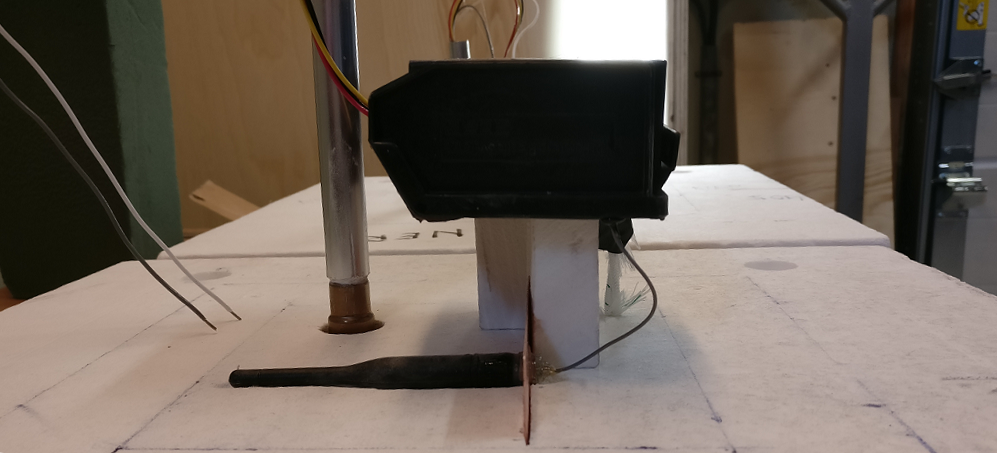
\includegraphics[width=.8\textwidth]{Chapter3/Figures/mechanical_construction.png}
    \caption{The mechanical design for the system.}
    \label{fig:mechanical_construction}
\end{figure}


\begin{figure}
    \centering
    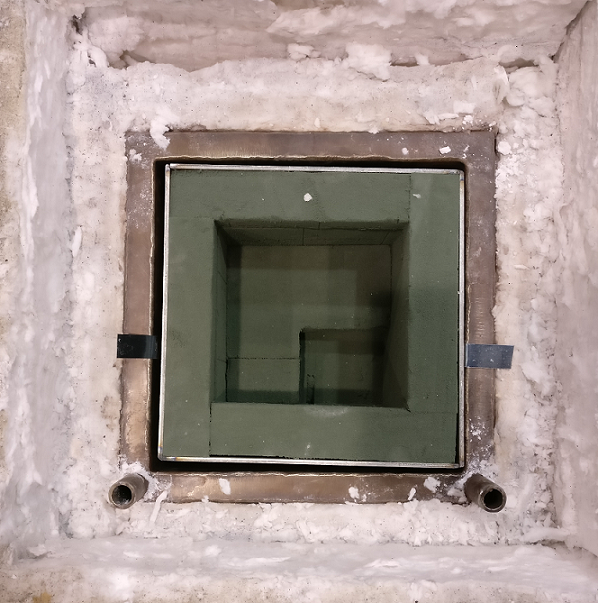
\includegraphics[width=.7\textwidth]{Chapter3/Figures/water_box.png}
    \caption{Metal box filled with flower foam and surrounded by high temperature isolation material.}
    \label{fig:water_box}
\end{figure}


\section{Controller for pumping current}

The pumping current has to be regulated so that the nernst voltage is stable at 450 mV. A controller is implemented for the current to hold this nernst voltage stable. On the first test at Mefos, a simple controller was used, which decreased or increased the current with fixed steps depending on whether the nernst voltage was higher or lower than 450 mV. This method worked fine in normal room conditions, where the oxygen level is stable and there is almost no disturbance. It didn't work well in the oven at Mefos where the conditions were a bit worse and there were faster changes in oxygen concentration.

For the second try a \ac{pid} controller was implemented. A \ac{pid} controller depends on three variables. The proportional error (P), the integrated error (I) and the derivative change of the error (D). When designing this controller, it was heavily weighted to depend much on the proportional error. At first, the I and D parts were set to be zero, and the P part was increased as high as it could before it started to oscillate. Then it was lowered a bit and the I part was increased a bit. The I part had some strict saturation limits to avoid overshoot and oscillation. It was mainly used to fine tune the current when the nernst voltage was close to 450 mV. Then the D part was increased until the controller started to oscillate, then lowered some. 


In the second small test at Mefos and the best test so far, a \ac{pi} controller was used instead. It is easier to tune than a \ac{pid} controller and it performed well enough for this application.




\section{O\texorpdfstring{$_2$} ~~calculations}


The oxygen concentration depends on the current drawn by the lambda sensor. When the nernst voltage is stable at 450 mV and the sensor has correct temperature, the relation between the current used by the sensor and oxygen concentration is described as figure \ref{fig:o2ipmeas}~\cite{LSU49}.


\begin{figure}
    \centering
    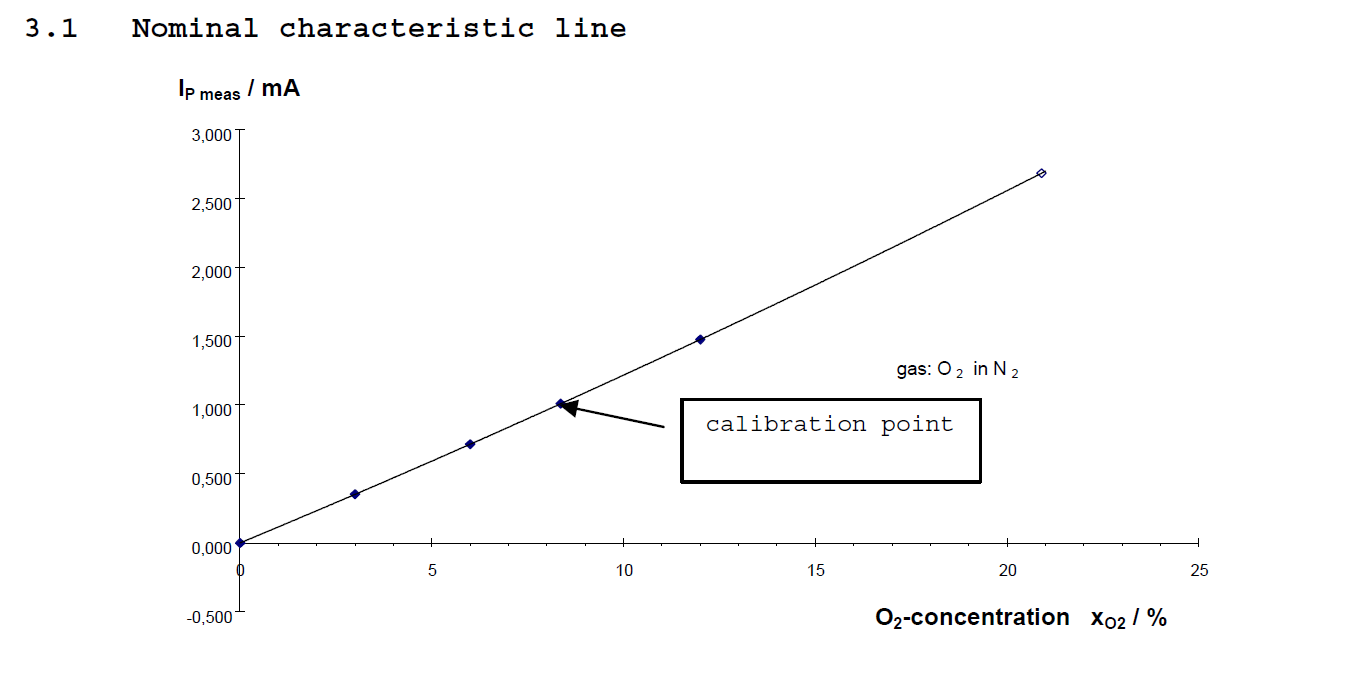
\includegraphics[width=\textwidth]{Chapter3/Figures/o2ipmeas.png}
    \caption{How the O$_2$ concentration depends on Ip$_{meas}$.\cite{LSU49}}
    \label{fig:o2ipmeas}
\end{figure}


Figure~\ref{fig:o2ipmeas} is provided from table~\ref{tab:o2ipmeas}, which is found in the datasheet for the lambda sensor~\cite{LSU49}. Ip$_{meas}$ is measured over a 61.9 $\Omega$ resistor, located in parallel with the trimming resistor calibrated for each lambda sensor in figure~\ref{fig:schematic_lsu49}.


\begin{table}
    \centering
    \caption{Relations between oxygen concentration and current used by lambda sensor.}
    \begin{tabular}{|l|r|r|r|r|r|r|} \hline
         O$_2$-conc. x$_{O2}$ [\%]    &  0    &  3.0 & 6.0    & 8.29  & 12.0  & 20.95  \\ \hline
         Ip${_meas}$ [mA]              &  0    & 0.33 & 0.67   & 0.94  & 1.38  & 2.54  \\ \hline
    \end{tabular}
    \label{tab:o2ipmeas}
\end{table}


\section{Software}

The software is designed for a PIC18F26K22~\cite{PIC18} and developed in MPLAB X IDE v3.51~\cite{MPLAB}.

\subsection{Overview}

Figure~\ref{fig:Software_map} gives an overview over the functionality of the software. At first, when the system starts, it initialises all the functions. It sets the pins to match its purpose, and initialise properties such as \ac{i2c}, \ac{adc} and \ac{pwm}.

Then while it waits for an \ac{i2c} interrupt from the radio unit, it constantly measures the nernst voltage to be able to control the pumping current for the sensor. If no \ac{i2c} interrupt happens within approximate 3 seconds, the system enters sleep mode. The system is brought back to an active mode when it receives an \ac{i2c} interrupt. When this happens, it sends its latest measured values from the nernst voltage, pumping current and \ac{pwm} amplitude through \ac{i2c} to the radio unit. The pumping current is used to calculate the oxygen concentration and \ac{pwm} amplitude for temperature calculations.

After the values have been sent, the system updates all values and then goes back to constantly measure the nernst voltage to regulate the pumping current for up to 3 seconds if no interrupt is received.

While the radio unit is active, it creates \ac{i2c} interrupts one time per second, and to ensure the sensor system is active during this time it waits 3 seconds before it enters sleep mode. When the sensor system enters sleep mode, it cut off the power to all components except the PIC. This is done by setting the gate high on a \ac{pmos}, which is used as a power switch.



\begin{figure}
    \centering
    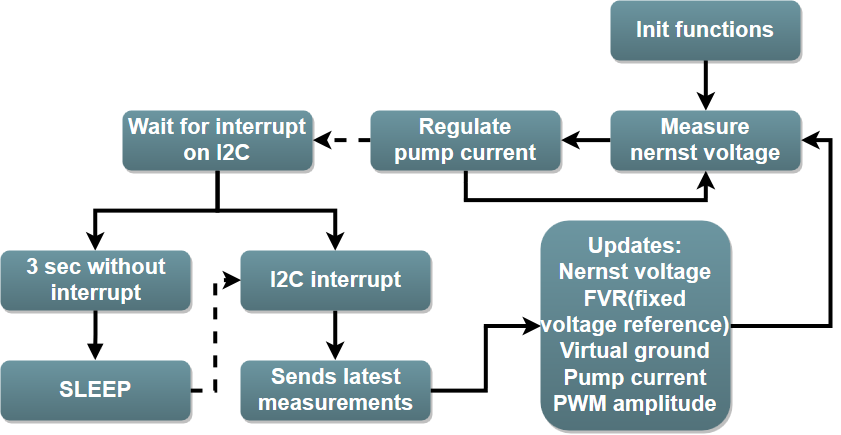
\includegraphics[width=\textwidth]{Chapter3/Figures/Software_map.png}
    \caption{Block schematic illustrating software functionality.}
    \label{fig:Software_map}
\end{figure}


\subsection{ADC measurements}

The \ac{adc} measurements which are done but not sent to the user, which also is shown in figure~\ref{fig:Software_map} is the \ac{fvr} and virtual ground. 

The virtual ground is measured to calculate the correct voltage difference entering the instrumentation amplifiers. This because the virtual ground is used on the reference pin on the instrumentation amplifiers. Then the output voltage is the voltage difference between the input signals added to the virtual ground. Then one has to subtract the virtual ground from the output measurement to be able to calculate the correct input difference.

The \ac{fvr} measurement is used to calculate the supply voltage for the sensor system. This voltage reference is set to be stable at 2.048 V, and by measuring the \ac{adc} value of this voltage, one can calculate which supply voltage is used. This is then used to compensate for differences caused by the supply voltage on the \ac{adc} measurements.



\subsection{Interrupt handler}

The interrupt handler has two different priorities. High and low priority.

An \ac{i2c} interrupt caused by the radio system generates a high priority interrupt and this communication is done within this high priority interrupt handler. Because this interrupt has the highest priority, all other interrupts happening during this time are put in a queue and is not handled before the high priority interrupt is done.


A low priority interrupt is caused by,

\begin{itemize}
    \item ADC conversion
    \item Timer4 interrupt
    \item Compare5 interrupt
\end{itemize}

The ADC interrupt is generated when a conversion is done and the ADC buffer holds a new 10-bit value. It then enters the low priority interrupt and clears the flag for ADC interrupt. The calculations for the ADC interrupt are then done in the main code.

When a Timer4 interrupt is generated it is done in the same way as the ADC interrupt, where it clear the flag and then returns to the main code, where calculations for the Timer4 interrupt are done. The Timer4 interrupt is used to start an ADC conversion on the nernst voltage.

The Compare5 interrupt is handled directly by the low priority interrupt handler. It is used to start an ADC conversion for the PWM amplitude, and the Compare5 register is comparing the clock value from Timer2 which is used for the PWM duty cycle and frequency. Then this Compare5 register guarantees that the ADC conversion for the PMW amplitude is done when the PWM signal is high and low to be able to calculate the amplitude of the signal.

\subsection{Measurement order}

\subsubsection{During the first test at Mefos}
When the sensor system is active and taking measurements, it will constantly be measuring the nernst voltage to be able to calibrate the Ip current which is used to decide what oxygen concentration it is in the environment.

When a request for data was received from the radio unit, the sensor system first sent it newest measurement values. Then it updated all values starting with the fixed voltage reference, followed by virtual ground, Ip current and temperature measurement. After this, it went back to calibrate the Ip current by constantly measure the nernst voltage. How often it measured the nernst voltage was decided by the Timer4 interrupt on the PIC. This interrupt was set to be generated 60 times per second.


\subsubsection{During the tests in the small oven at Mefos}
The measuring order was changed a bit in these tests, compared to the previous. One difference was that the temperature was only measured one fifth of the times compared to the other measurements. The generated PWM signal was only activated during this measurement. The reason for this was to decrease the potential of noise on the other measurement being caused by the PWM signal.

The other difference during these tests was the number of measurements. This time each measurement, except for the nernst voltage, was done 8 times between each I2C request. The mean value from these measurements was sent to the user. The nernst voltage was measured continuously during all time the system was active. When the nernst voltage was sent to the user, it was the mean value from 8 of the measurements between the I2C requests. At the first test, only one measurement was considered when it was sent to the user.



\section{Test and fault search on system}


When everything was built together and the system was tested in normal tempered air and heated up with a power supply, it didn't work. The nernst voltage was at its bottom and the \ac{dac} didn't increase the current. Some temperature cycles on the sensor were then made with a power supply. The temperature was changed in such a way, the sensor went from not operating temperature to operating temperature for some iteration and it started to work after a while then.


This caused some major concerns however the system would be able to run in the oven or not. 

By doing some fault search and attempts to recreate this error, it seemed at that moment like the sensor system had a lower chance of running correctly after it waked up from sleep mode. 

At the test day with this information, the sensor was heated up with a power supply and confirmed it operated correctly. Then it was left in its active mode during the rest of the time before it entered the oven and inside the oven as well.


The fault searching continued after the test and it turned out that the error was within the software for the current regulator. It caused an overflow on the 12-bit \ac{dac} value, where the software thought it was sending its maximum value, but this value was 0 V for the \ac{dac}.


%When the two setups of sensors was first run in Kalix, it didn't work from start. But after some mixture with the temperature, both system started to give good oxygen values. In these cases it seemed like they started to give correct values on a sharp temperature rise event on the sensor.

%These tests in Kalix was on a Friday and the setups were tested once more in Lule\r{a} on Monday and for the first system it didn't worked at first. But after some temperature cycles it started to work. But this time it started to give good values when the temperature already was high and not during a sharp temperature change and that was for the tag 1ADF

%On the next sensor setup it will be tested if the system will start working if it is left with a high temperature for a while, without changing the temperature or anything when it already is high. This system have the tag 1ADE

%The other system start working immediately on the Monday trial and it have the tag 1ADE 


%There were some thoughts that some contaminants might have damage the sensors, during the mechanical built up phase. The sensors were mounted to the isolation material with a epoxy and soft isolation material. Therefore we used a test sensor that was mounted to a test piece with the same method and afterwards the sensor still worked, which lowered the change for the epoxy to damage the sensor.

%After some readings that silicon is harmful for the sensors, a similar test was performed where the sensor had to "breathe" silicon for 15-20 minutes before it were tested. Silicon were used in our case to mount a aluminium pipe to the sensor, which would increase the cooling performance for the sensor. The sensor stilled worked after this test also though. 

%The fault searching resumed after the test with the debugger connected to the system. The error were reproduced after some heating cycles. When it was reproduced, the bias points were measured with a oscilloscope and it turned out that the fault was in the software controller for the pumping current. It caused an overflow to happen, which caused the DAC to send out 0 V instead of 5 V.


\section{Preparations for a test in a small oven at Mefos}

The main goal of this test was to see that the electronics for the oxygen measurement behave as wanted, when the sensor was in a rough environment, as this created the most concerns after the previous test. The sensor and electronics did survive in the first test and this was promising. When the oxygen values from the lambda sensor were compared to the oxygen values from the already integrated BOSCH sensor, it was more noise from the lambda sensor. Both measurements could be the truth however, because the BOSCH sensors measure the values from a well-mixed gas, where it isn't rapid changes in oxygen concentration.

So even if the oxygen concentrations around the lambda sensor have a high variance, the nernst cell which is supposed to be held at 450 mV should be stable. It wasn't stable in the test, and because of this, it is not ideal to say that the oxygen concentration measured by the lambda sensor are a good representation of the truth. This variation is the main reason a better controller has to be implemented.

The goal with this smaller test at Mefos is to get verification, that a better controller has been implemented.




\makechapter{Result}{Result\label{ch4}}
\section{First test in oven}

The first trial in the oven took place 2017-03-28 at Mefos in Lule\r{a}. The data communication worked during the time in the oven, where the data could be followed using Electrotech's radio antenna and serial communication.

When heating up the oven, it didn't reach its expected temperature in time. This caused some delays and the sensor was then placed in the oven 3 hours later than planned. This gave us the opportunity to do some fault searching for the sensor, which stopped working sometimes for unknown reasons. However what seemed like a pattern was that the sensor system started to fail during the heat up process after it entered sleep mode.


Because of this, the sensor was heated up with a separate voltage cube and made sure it gave some valid data before placing it into the oven and the system was never reentering sleep mode after this heat up process.


Just the tip of the sensor was pointing out from the isolation material and had direct contact with the oven's environment. It took about 10-15 minutes for the sensor to reach its operating temperature and this time could be decreased by either expose a bigger part of the sensor to the oven or preheat the sensor with a gas burned or similar. However, by exposing a bigger part of the sensor to the oven, it will most probably decrease its lifetime.

\begin{figure}
    \centering
    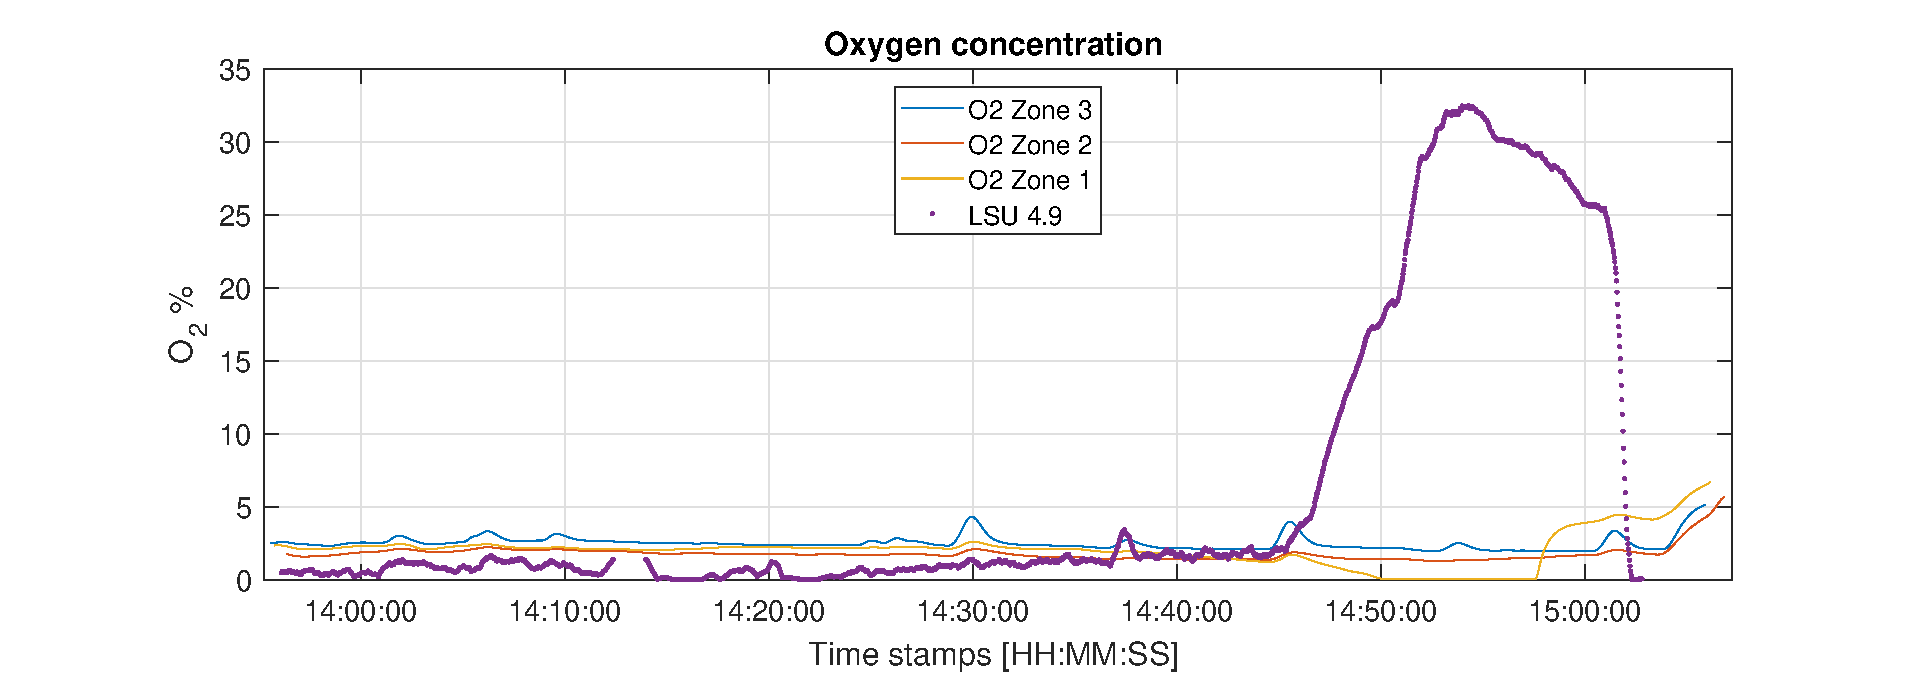
\includegraphics[width=\textwidth]{Chapter4/Figures/syre_dots.eps}
    \caption{The oxygen level during the test.}
    \label{fig:syre_dots}
\end{figure}

\subsection{Measurements during the first test.}

Figure \ref{fig:syre_dots} shows the oxygen values measured by the lambda sensor during its time in the oven. There are also three lines with reference measurements. Exactly what time the sensor went from one zone to another is hard to tell. But the time in each zone was the same, where it started in zone 1. There is also a gap with no data in this graph. This is due to unreliable data and therefore neglected. The oxygen calculations are not correct when the lambda value is below 1, which represent a negative current on the pumping current, and that most probably what happened.

In figure \ref{fig:nernst_both} there are two lines made by the same data. Both lines show the voltage drop over the nernst cell during the time in the oven, where the orange line is mean value by nearby data. This voltage is supposed to be 450 mV and from the beginning it was below this limit. This time was before the sensor reached its operating temperature.


\begin{figure}
    \centering
    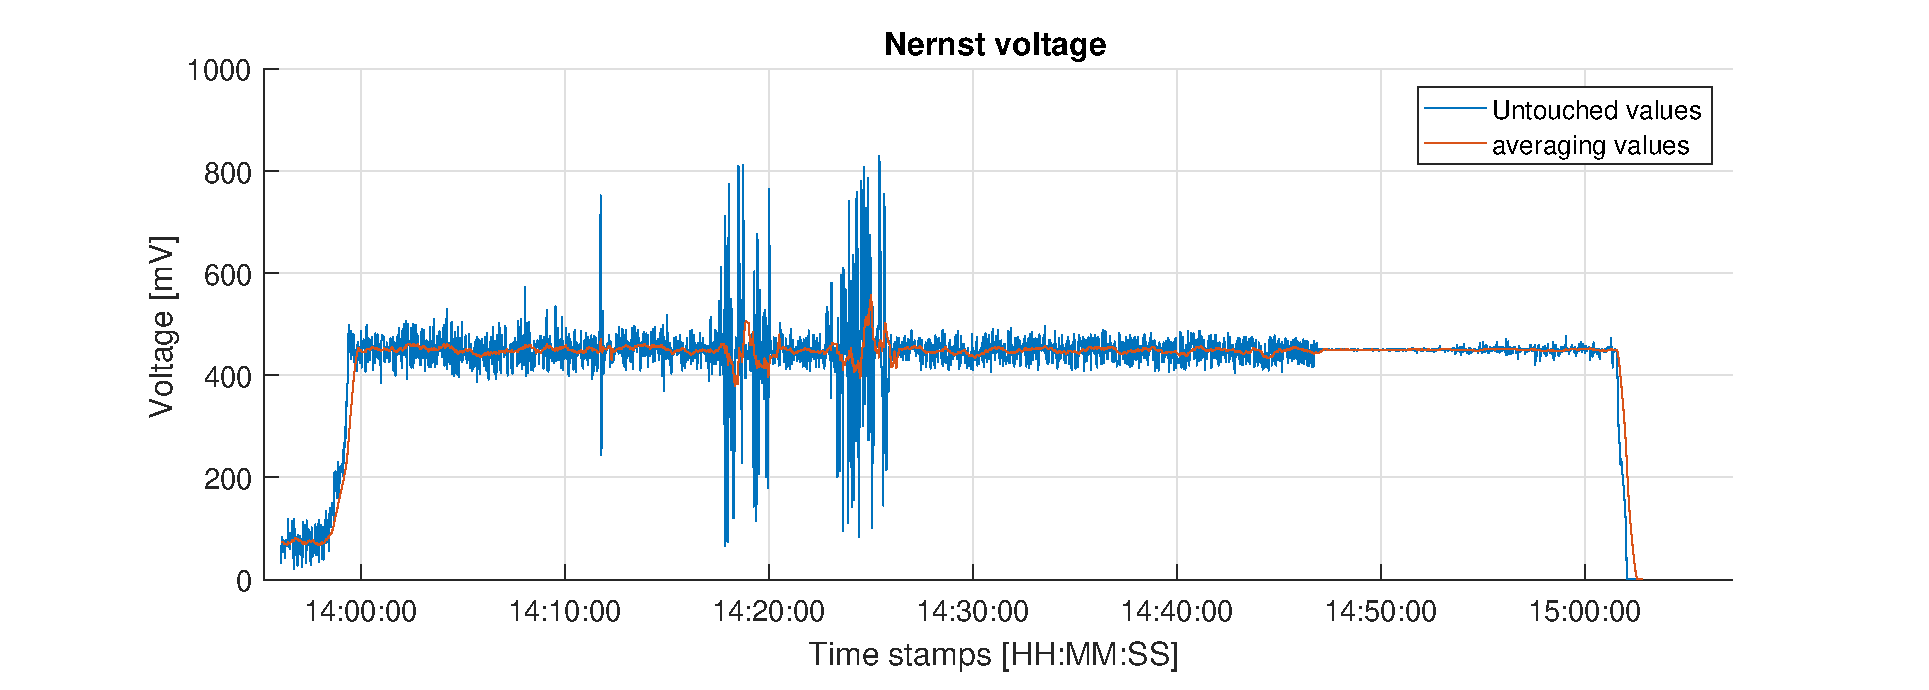
\includegraphics[width=\textwidth]{Chapter4/Figures/nernst_both.eps}
    \caption{The voltage over the nernst cell during the test.}
    \label{fig:nernst_both}
\end{figure}

Figure \ref{fig:temperature_both} also have two lines done with same data. The blue line is untouched values and the orange is the mean value of nearby measurements. Figure \ref{fig:temperature_both}, shows the temperature of the sensor during its time in the oven and this temperature is calculated by measuring the resistance over the nernst cell.





\begin{figure}
    \centering
    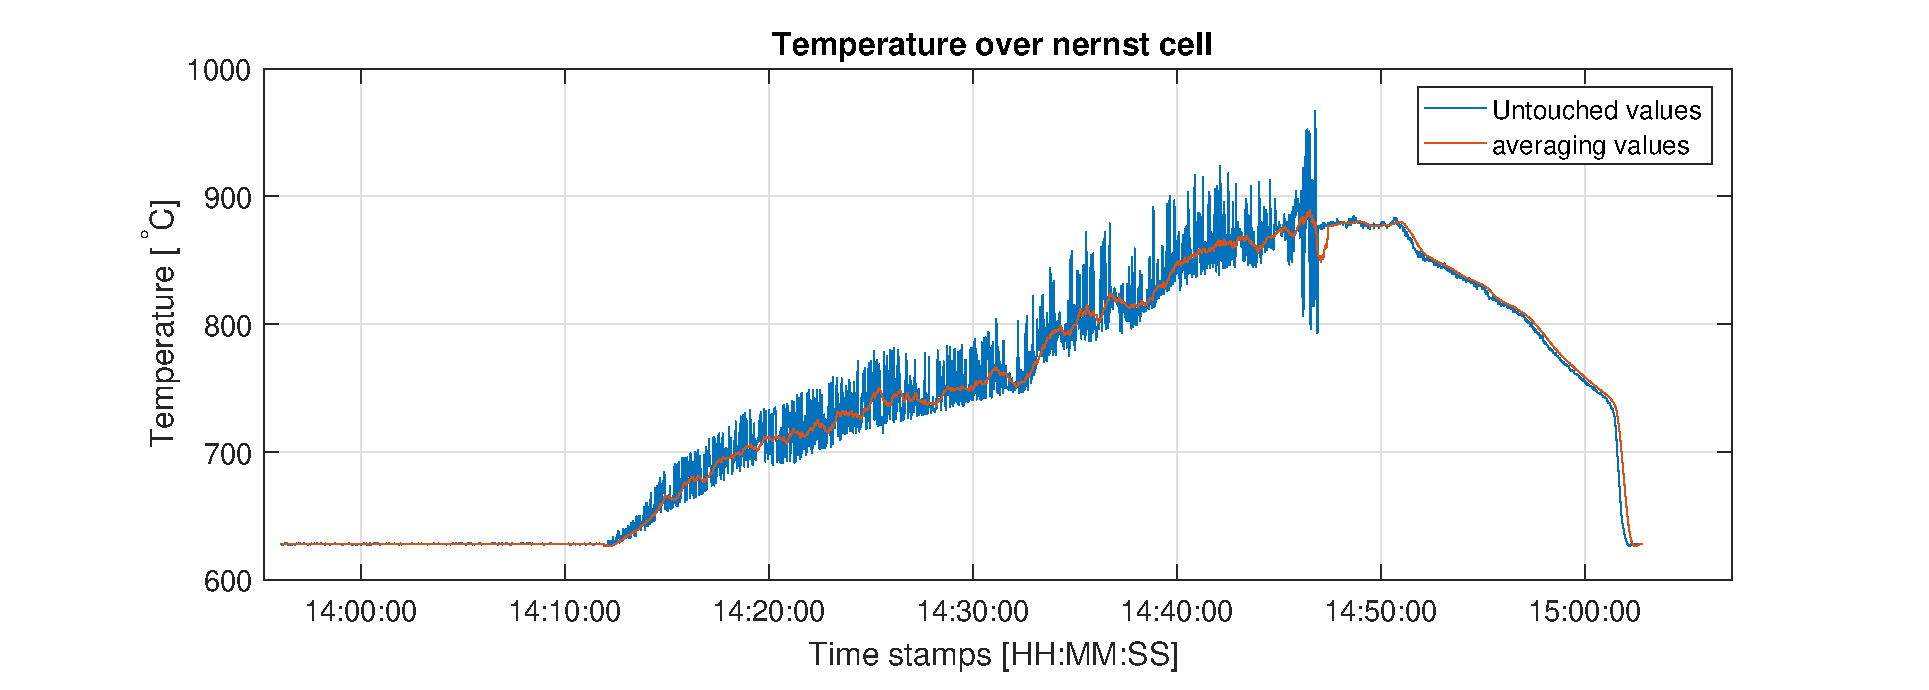
\includegraphics[width=\textwidth]{Chapter4/Figures/temperature_both.eps}
    \caption{The PWM temperature measurement during the test.}
    \label{fig:temperature_both}
\end{figure}


\subsection{Day after test}

The day after the first test was performed, the lambda sensor with its electronics was collected and brought back to \ac{ltu}. Because the water only reached 70 degrees, the electronics and the mechanical design still looked to be in good shape. There was still some power in the batteries and Electrotech's radio system still sent data, which were collected by the antenna. The sensor was then heated up with a power supply and when it reached its operating temperature, it started to send correct oxygen concentration for the room.

So the system did survive the 2 hours in the oven and could then be re-used. At least the electronics could be re-used, without any risk. But how much the time in the oven shortened the lambda sensor's lifetime is hard to tell though.



%\section{Small tests at Mefos}
\section{Tests in small oven at Mefos}

\subsection{First test 20170412}

This test was done in a small oven heated up to 1200 $^\circ$C. The lambda sensor was then put in the oven through a small hole and it reached its operating temperature fast. The temperature of the sensor kept increasing until it broke however, so this sensor only managed to give data for a short amount of time before it broke down.

Another lambda sensor then replaced this sensor. The resistance on the electronics was calibrated for the first lambda sensor, so the values of the second sensor were a bit shifted. This sensor was not placed as deep in the oven as the first sensor. So this time the sensor survived much better and gave valid data. The values seemed to have an offset compared to the reference measurement and it was a bit noisy as well. If the condition in the oven was changed, the lambda sensor and reference sensor changed in the same way. But it was still an offset error by a factor of about 3.

After some changes of the oxygen levels, it was a plan to change the regulator of the nernst voltage a bit and the programmer was placed to the electronics. Immediately when the programmer was connected both the oxygen and nernst measurement become more stable. But it still had an offset, which seemed to change a bit.




\subsection{Second test 20170420}

The changes in this test compared to the first test in a small oven, were that the position of the reference measurement for the oxygen was changed and the controller for the pump current was slightly changed.

The previous time, the reference measurement was placed at the top corner of the oven. This was a bigger hole compared to the one where the lambda sensor was placed. This measurement was moved to the same hole as the lambda sensor this time and it made a big difference in the oxygen concentration for the reference measurement. This hole is placed in the middle of a wall of the oven.

\begin{figure}
    \centering
    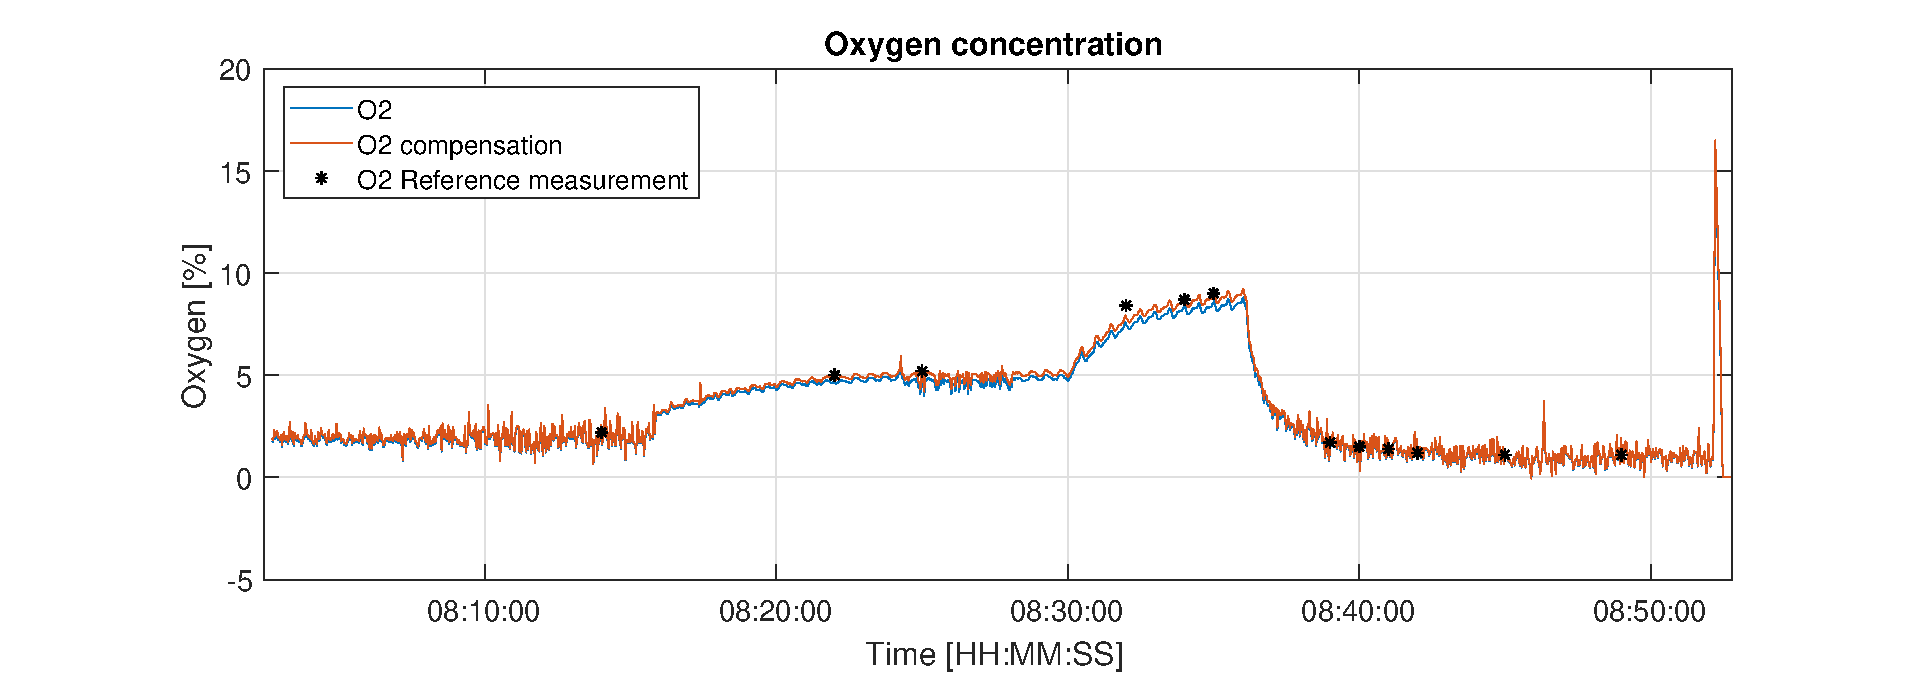
\includegraphics[width = \textwidth]{Chapter4/Figures/oxygen_second_small.eps}
    \caption{Oxygen measurement in small oven with reference points.}
    \label{fig:oxygen_second_small}
\end{figure}

In figure \ref{fig:oxygen_second_small} and \ref{fig:nernst_second_small} one can see that the measurements are clearly more stable at two time intervals. During these intervals, the sensor was also heated from a voltage cube and not only from the heat produced by the oven.

The reference measurement in figure \ref{fig:oxygen_second_small} was performed by a separate unit, which didn't log the measurement data and test points was then noted now and then manually.

\begin{figure}
    \centering
    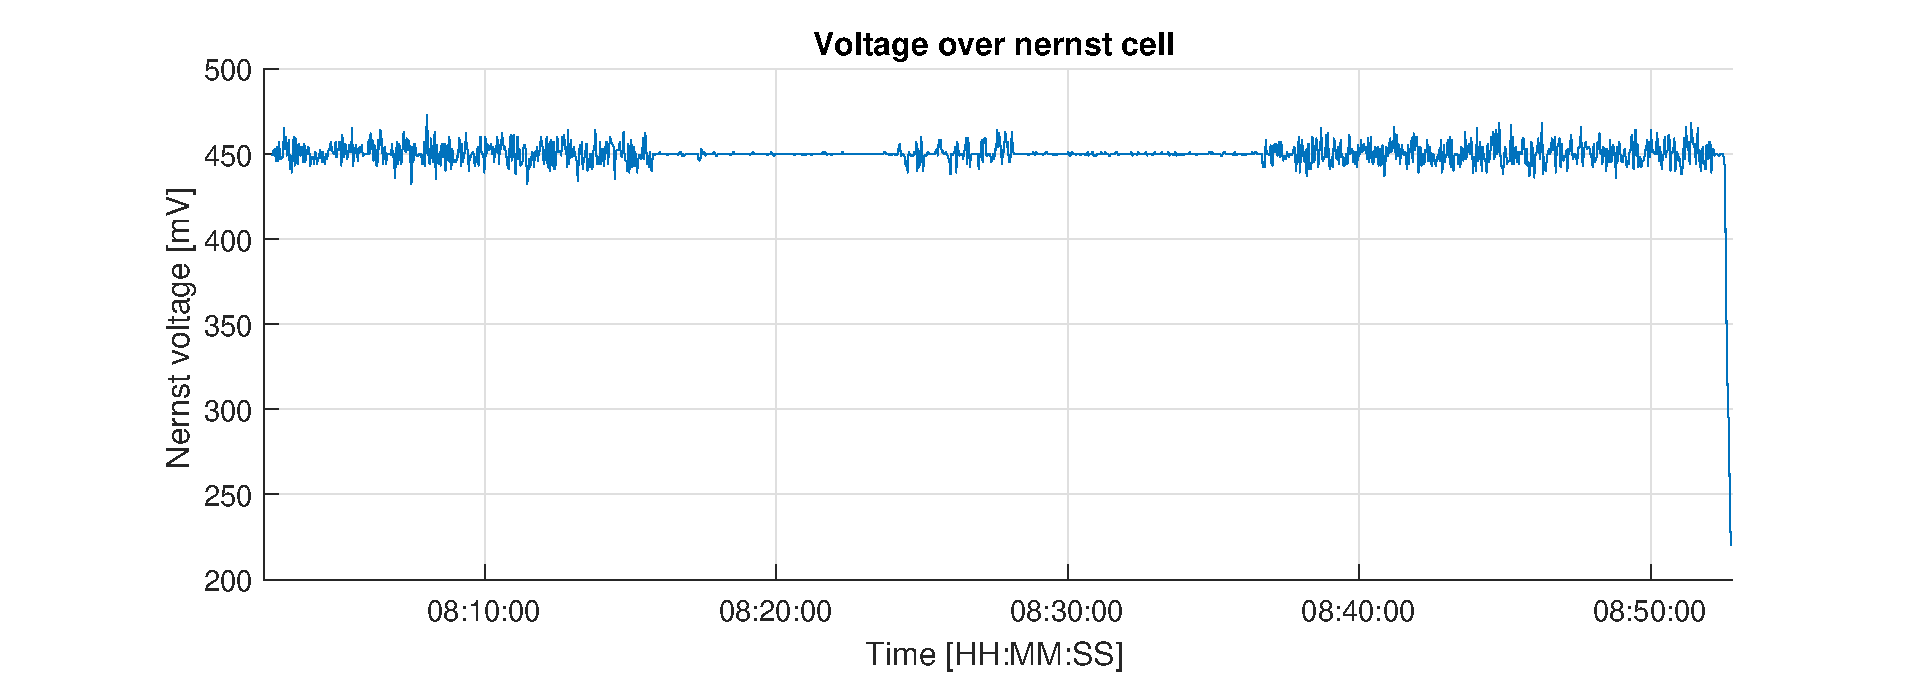
\includegraphics[width = \textwidth]{Chapter4/Figures/nernst_second_small.eps}
    \caption{Voltage drop over nernst cell at the test in a small oven.}
    \label{fig:nernst_second_small}
\end{figure}

The temperature measurements in figure~\ref{fig:temperature_second_small} are done by measuring the resistance over the nernst cell. These temperature measurements are valid from approximate 630 $^\circ$C and above. The actual temperature is most likely below this temperature when the measurement is stable at 630 $^\circ$C for longer times.


\begin{figure}
    \centering
    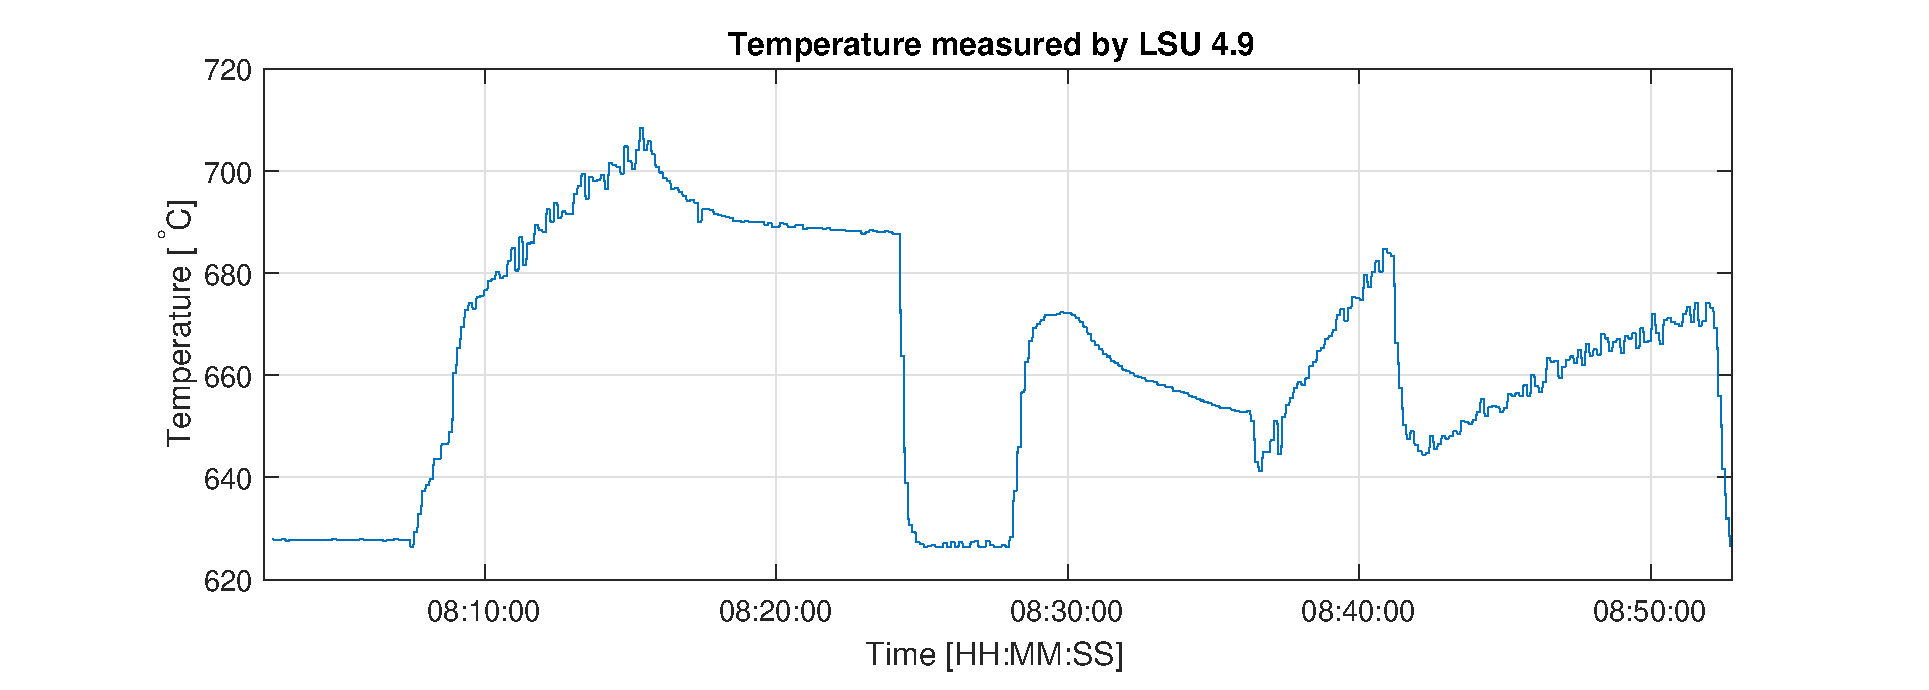
\includegraphics[width = \textwidth]{Chapter4/Figures/temperature_second_small.eps}
    \caption{Temperature measurement at sensor element.}
    \label{fig:temperature_second_small}
\end{figure}



\makechapter{Discussion}{Discussion\label{ch5}}

\section{Hardware design}

\subsection{PCB design}

From the beginning, the plan was to order two sets of PCBs. When the first design arrived, plans were changed and a second order should only be done if it was really needed. The first design contained some design errors and it had to be some patches to the PCB before it behaved as expected. A number of errors would maybe be decreased if the first design wasn't as rushed as it was. This also showed that even if it would be two iterations of PCB designs, longer time should have been spent to verify the first design's functionality.

To not put a LED on the PCB was a bad idea. It was skipped to hold the current consumption down, but you don't have to use it during the real experiments. It is a good source when debugging and that's why it should be implemented. Also, a LED with low power consumption could have been chosen.


\subsection{Functionality}

That the sensor was designed to handle some variance on the operating voltage was good. It made it easy to go from unregulated 3.6 V to 5 V regulated. If the system would have been designed to handle only for example 3.3 V and we would found out in Kalix it was more beneficial to run it on 5 V, due to battery limitations, it could create big troubles if it wasn't that easy to change to 5 V.


I still think it would be the best to run the sensor on 3.3 V in the end.  This would simplify the integration part of the sensor and radio unit. Also, I don't see the point of running the sensor on 5 V when it most likely can run on 3.3 V without any trade-offs on functionality, more than it gets a bit worse measuring range. But the range available with 3.3 V is most likely good enough in the oven. It will then not be able to measure lambda value far below 1. But when it is used in this application, it is supposed to measure lambda values from 1 and above. If it goes far below 1, there is a bad combustion in the oven.

A possible rework to improve its functionality on 3.3 V is to have two virtual grounds. One for the sensor and one for the reference points on the instrumentation amplifiers.

When the sensor runs on 5 V, it is good to have the virtual ground in the middle which is 2.5 V. But when it run on 3.3 V, it is preferable to have the virtual ground around 1 V. But for the instrumentation amplifiers it is better to have the reference point in the middle, which is 1.65 V at 3.3 V.



\section{Thoughts after first test}

Even if the result from the first test left some concerns because of unstable values, it was promising that the most critical functions worked. The fact it did survive all time in the oven and sent data without interruptions was justifying. Also, the stuff that didn't work as expected felt doable to give some rework and patches.

Also when looking into the smaller test, where it made a huge difference on the oxygen concentration depending on which location we were measuring, it felt like the values measured by the lambda sensor could be correct also in the first test. 

It is interesting though that the oxygen level went really high at the end of the experiment and the sensor still worked when it was tested the day after. When the oxygen level did go away like that, the sensor was passing the burner. Either this burner or the environment in the oven caused the sensor to behave in a bad way, or it was a really high oxygen level because of a lot of unburned oxygen in this spot. But the later seems unlikely due to air is added as an oxygen source for the combustion and therefore it wouldn't be able to reach over approximately 21 $\%$ oxygen.

\section{Tests in small oven at Mefos}

\subsection{First test in small oven}

This test was mostly done to give a confirmation that the system worked as expected. The software was heavily reworked since the first test and it worked well on the lab-bench. It did give more stable values than the first test, but it was still some noise.

The actual oxygen level didn't match well at all either. It was roughly a factor 3 off and this left the most concerns if some crucial mistakes were made.


\subsection{Second test in small oven}

In this experiment, the pump current regulator has changed from a \ac{pid} controller to a \ac{pi} controller. In theory a \ac{pid} controller should be better, but a \ac{pi} controller is easier to tune. The values in this experiment did not oscillate as much as it did in the previous test. But the oxygen level was still off at the beginning of the measurements.

The reference measurements and the lambda sensor measurements had different locations, after assuming same conditions on both places. To verify this, the reference measurement changed to the same spot as the lambda sensor instead and they now showed the same values.



\section{Conclusion}

The measurement and encapsulation principle has been shown to work in the intended application. It is clear that a possibility exists to migrate the results from this work into a product. This will aid in process understanding and energy usage optimization.

However, There is still room for improvements on this product. A better current regulator should give a more stable measurement of the oxygen value. But the concept of using instrumentation amplifiers has been a good method. It was useful for saving pins on the \ac{mcu}, its simplicity to use and still get an accurate differential gain. Of course one could change to higher resolutions on the \ac{adc} channels, but in my opinion, 10-bits is enough for this kind of application.

%The DAC could have a higher resolution however. 12-bit is fine, but going up to maybe 14 or 16 could make some difference.

Maybe there should be some more work to run the sensor on a lower voltage, which doesn't seem to be impossible at all. 





%%==================================================================
%% Include bibliography references here
%% Replace the "thesisreferences" with your
%% own reference database
%%==================================================================
\bibliographystyle{unsrt}

\fancyhead[LO]{}%
\fancyhead[RE]{}%
\fancyhead[LE]{\thepage}%
\fancyhead[RO]{\thepage}
\bibliography{thesisreferences}



%%==================================================================
%% Include any appendices here.
%%==================================================================
\appendix % This command initializes the appendix part, Don't change!

\makeappendix{Appendix C}{Abbreviation list\label{appC}}
%Least squares fit of response surface
%models by multiple linear regression\label{appA}}

\printacronyms[include-classes=abbrev,name=Abbreviations]




\makeappendix{Appendix A}{Full schematic for PCB design\label{appB}}
%Least squares fit of response surface
%models by multiple linear regression\label{appA}}


\begin{figure}[h]
    \centering
    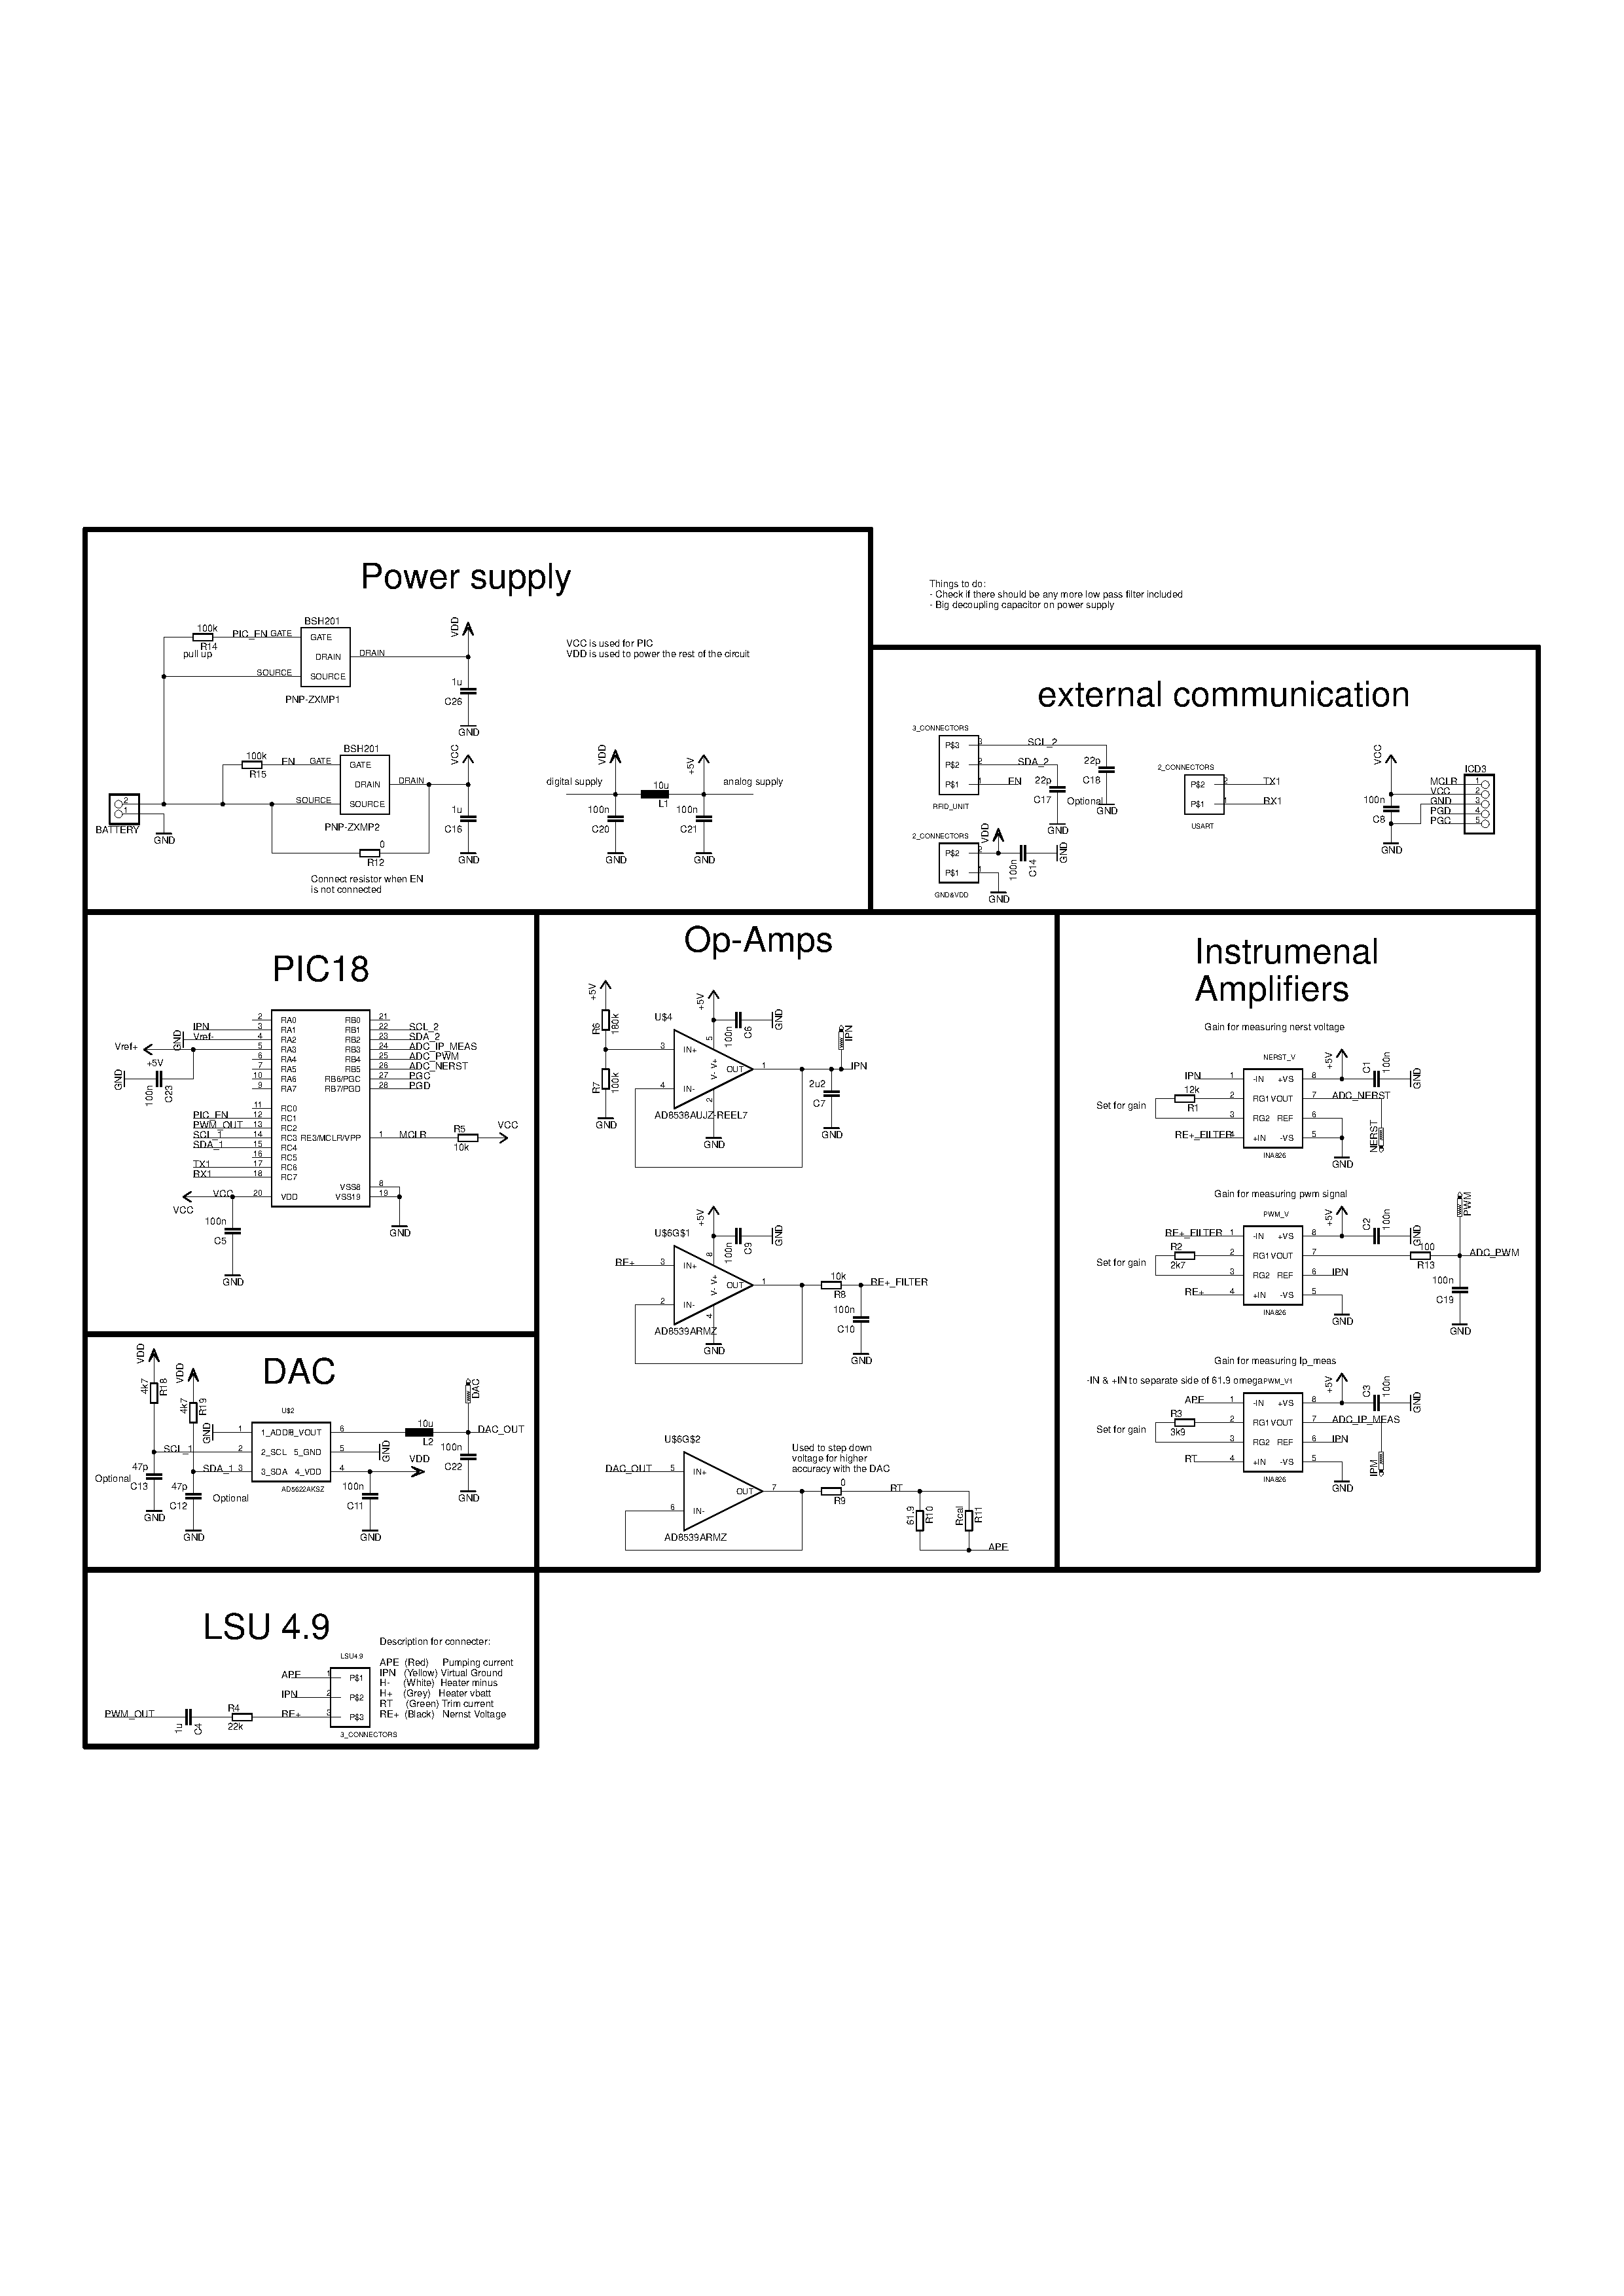
\includegraphics[width=.94\textwidth]{Figures/Lambdasond_schematic.pdf}
    \caption{Full schematic for final PCB design.}
    \label{fig:Lambdasond_V1.1schematic}
\end{figure}

%% Include appendix A, add more if needed
\makeappendix{Appendix B}{C code designed for PIC18F26K22 controlling LSU4.9\label{appA}}
%Least squares fit of response surface
%models by multiple linear regression\label{appA}}




\lstinputlisting[language=C]{Appendices/main.c}
\lstinputlisting[language=C]{Appendices/main.h}

\lstinputlisting[language=C]{Appendices/ADChandler.h}
\lstinputlisting[language=C]{Appendices/ADChandler.c}

\lstinputlisting[language=C]{Appendices/I2Chandler.h}
\lstinputlisting[language=C]{Appendices/I2Chandler.c}

\lstinputlisting[language=C]{Appendices/INTERRUPThandler.h}
\lstinputlisting[language=C]{Appendices/INTERRUPThandler.c}

\lstinputlisting[language=C]{Appendices/PWMsteering.h}
\lstinputlisting[language=C]{Appendices/PWMsteering.c}








\end{document}
